\chapter{场景仿真、方案对比与在线策略验证}
\label{chap:simulation}

本章对第四章建立的联合调度模型进行数值验证。验证分为三部分：首先通过合成48~h序列检查
功率平衡、状态递推和各输出通道的运行逻辑；随后在同一正常48~h窗口内比较纯电、纯氢、纯算
和在线协同四类方案；最后采用8,760~h连续序列检验在线策略的状态继承、极端事件响应和求解稳定性。
不同时间尺度的结果分别讨论，以保持机制验证、方案比较和年度运行分析的统计含义一致。

本章数值结果均由模型仿真得到。资源数据中只有NASA POWER风速、辐照度与
气温等属于政府科研机构公开代理数据；设备容量、价格、惩罚系数、潮流速度、事件参数、储备目标和排放因子采用本研究的基准参数。公开网格数据并非项目测风、测光或海洋实测，因而
无法直接形成场址资源评估、工程定容、投资决策或可靠性承诺。

\section{验证逻辑与第4章模型映射}

\subsection{分层验证框架}

仿真按照“机制验证--典型窗口比较--年度连续验证”三个层次组织，各层的时间范围、输入数据和评价指标见表~\ref{tab:c5-evidence-levels}。

\begin{table}[htbp]
\centering
\caption{三类仿真的时间范围与评价内容}
\label{tab:c5-evidence-levels}
\begin{tabularx}{\textwidth}{p{2.5cm}p{2.6cm}p{3.3cm}X}
\toprule
验证层次 & 时间尺度 & 主要输入 & 评价内容\\
\midrule
合成机制验证 & 48~h、8个阶段 & 人工构造风光潮、任务、价格和通道状态 & 全通道能否激活；母线、BESS、氢库存、服务账是否闭合；突升突降是否触发预期动作\\
正常典型比较 & 48~h、正常状态 & 从年度正常候选中离线选取的同一多源窗口 & 三类资产基准与在线策略在共同短窗口下的消纳、产品输出、ENS及运行层价值差异\\
年度在线验证 & 8,760~h、逐小时连续 & 年度公开资源数据、内部潮流序列、价格负荷及构造的台风压力测试 & 非前视预测、状态继承、事件收缩--恢复、最小ENS层级能否全年运行\\
\bottomrule
\end{tabularx}
\end{table}
\sourcetype{项目内部测试架构；所有场景参数均按其数据来源单独标识。}

合成48~h场景用于模型验证，不参加方案排名。横向比较只使用正常典型48~h。年度层按
既定范围只运行在线先验--后验策略，不重算三个资产基准。因此，年度层没有“相对纯电提高
多少”的有效结论；任何年度基准旧表、22种固定比例方案和完美预见全时域结果均退出本章
验证框架。

\subsection{第4章--第5章可追溯矩阵}

表~\ref{tab:c4-c5-trace}列示第四章各模型在本章仿真中的实现程度，以区分完整模型结构与本轮计算采用的简化形式。

\begin{longtable}{p{1.4cm}p{3.0cm}p{5.6cm}p{4.0cm}}
\caption{第4章模型与第五章测试的可追溯关系}\label{tab:c4-c5-trace}\\
\toprule
第4章 & 理论模型 & 本章仿真实现 & 验收指标\\
\midrule
\endfirsthead
\toprule
第4章 & 理论模型 & 本章仿真实现 & 验收指标\\
\midrule
\endhead
4.2 & 风、光、潮设备及源侧聚合 & 680/80/40~MW三源装机；可用功率由逐时资源与4.3设备模型计算，不预设总发电量 & 三源逐时可用功率、总可用电量、可用=利用+弃电\\
4.3 & 海缆、氢、算力及海洋用能供给 & 海缆采用8\%固定损耗；氢气供应为逐时等效管输/船运；未建氨系统 & 送受端电量、氢提取/供应、算力服务与海洋服务分账\\
4.4 & BESS与构网代理裕度 & 80~MW / 160~MWh、充放效率0.95、SOC 0.10--0.90，并保留5~MW/1~MWh上下构网代理裕度 & SOC、充放互斥、状态递推、有效SOC边界0.10625--0.89375\\
4.5 & 电解、储氢及可选氢转电 & 5$\times$20~MW PEM、固定SEC 56.77~kWh/kg、72,000~kg库存；年度启用30~MW氢转电额定通道但无场外补氢 & 机制场景产氢/供应；年度氢库存、产用和氢转电自然结果\\
4.6 & 算力任务、设施功率、PUE与SLA & 本轮联合MILP采用聚合设施功率、柔性上界和给定逐时PUE；未嵌入详细任务队列、动态热状态和逾期约束 & 设施输入、MWh-CS服务、等效周期PUE、基础算力ENS\\
4.7 & 公共母线功率平衡 & 源侧利用+BESS放电+氢转电=充电+电解+算力+海缆+海洋服务+内部已供负荷 & 最大母线残差、弃电与关键ENS互斥、独立审计\\
4.8 & 经济、环境和可靠性 & 运行净成本、确定性ENS和运行层温室气体代理；未做CAPEX、NPV和完整LCA & 收入/成本分账、ENS分负荷、项目/避免/净排放代理\\
4.9 & 逐时E/H/C计划与可行域 & 计划份额只作用于当前小时实际可选投入，不使用全期总供电量；允许可靠性优先时释放 & 计划偏差、释放小时、资产开关与无固定比例审计\\
4.10 & 因果求解及动态复核门 & 当前为1~h单步在线计划与结算；状态逐时继承；不等同于多小时MPC或构网动态验证 & 信息边界、8,760小时求解状态、REGFM、EMT和HIL后续验证内容\\
\bottomrule
\end{longtable}
\sourcetype{项目联合仿真程序及结果账本。表内参数按场景设定。}

上述映射揭示三项需要特别约束表述的实现差异。其一，第4章4.6的任务队列和动态PUE是
完整聚合模型，本章基准仿真采用聚合算力接口；其二，第4章规划级海缆损耗可采用分段线性
模型，基准仿真采用8\%固定损耗；其三，第4章完整氢库存式保留安全放散变量，本章仿真没有
单列放散，等价于放散为零并由源侧弃电处理不可利用电量。这些差异已经在第4章相应小节
明确，相关差异在结果解释中分别说明。

\subsection{统一结果判据}

逐时结果在满足以下条件后纳入统计：求解器返回可用整数最优解；公共母线、
BESS状态、氢库存、海缆受送端和服务账残差均在数值容差内；容量、SOC、库存、互斥、
资产开关和逐时计划约束没有越界；当前小时末状态原样传递给下一小时。确定性单时序缺供
统一称为ENS，只有给定多场景概率时才可称EENS，定义遵循第4章式~\eqref{eq:ens}--
\eqref{eq:eens}及ENTSO-E方法口径\cite{entsoe-maf}。

小时MILP的审计通过只证明能量与逻辑可行，不足以证明频率、电压、故障穿越、黑启动、海工
抗台风、通信SLA或船运计划合格。构网型储能在小时模型中只表现为上下有功和能量裕度，
相关动态性能仍需通过REGFM、EMT、HIL和现场试验验证。

\section{数据、容量与场景构造}

\subsection{共同资产与计量边界}

当前机制配置采用800~MW多源装机，其中风电680~MW、光伏80~MW、潮流能40~MW，名义
容量比例为85\%/10\%/5\%。产品侧包括200~MW海缆送端、100~MW模块化电解槽、
120~MW算力设施、18~MW海洋刚性负荷，以及80~MW / 160~MWh BESS。上述容量用于构造多通道竞争的基准算例，未对应国家能源集团的特定工程，也未通过容量优化获得。

\begin{table}[htbp]
\centering
\caption{基准仿真的共同设备参数}
\label{tab:c5-common-config}
\begin{tabularx}{\textwidth}{p{2.5cm}p{4.0cm}X}
\toprule
对象 & 当前参数 & 证据与状态\\
\midrule
源侧 & 风680、光80、潮40~MW & 本研究基准参数\\
BESS & 80~MW / 160~MWh；$\eta_{ch}=\eta_{dis}=0.95$；SOC 0.10--0.90 & 本研究基准参数\\
构网代理裕度 & 上下各5~MW / 1~MWh & 用于小时级备用分析，具体数值需结合PCS参数和系统扰动校核\\
PEM与储氢 & 5$\times$20~MW；SEC 56.77~kWh/kg；72,000~kg & SEC满负荷取值参考制造商资料；部分负荷效率和库存参数采用基准值\\
海缆 & 送端200~MW；受端损耗率8\% & 本研究基准参数，后续依据海缆方案和负载特性更新\\
算力 & 设施上限120~MW；16个聚合模块；逐时PUE输入 & 本研究基准参数；PUE定义依据行业组织和政府资料\cite{green-grid-pue,doe-pue}\\
海洋用能 & 刚性需求18~MW & 本研究基准负荷，后续依据具体用能对象和负荷曲线更新\\
\bottomrule
\end{tabularx}
\end{table}

模型把“内部关键负荷”定义为源侧辅机、0.25~MW公共辅机和0.20~MW POI后固定损失等
已建字段之和，而非完整能源岛酒店负荷、消防、淡化、通信和安全系统清单。18~MW海洋
用能另列刚性负荷。年度算力全部设置为可中断柔性负荷，基础算力需求为零；因此年度算力
未执行不会计入ENS。若未来存在不可中断客户SLA，需恢复基础算力或任务队列场景，无法
沿用本章零基础算力ENS结论。

\subsection{年度多源资源数据与代理限制}

年度风速、地表短波辐照和气温来自NASA POWER 2025年逐时点数据\cite{nasa-power}，
坐标为北纬21.2$^{\circ}$、东经113.0$^{\circ}$，时标为UTC。该来源属于政府科研机构公开
数据，但并非项目场址测量。源侧发电量由逐时资源输入和第四章设备模型共同计算，并受装机容量约束，
由功率曲线、状态机、辅机和损耗计算得到，再受装机上限约束。

当前资源处理仍存在三个显著限制：
\begin{enumerate}[label=(\arabic*)]
\item NASA 50~m风速直接进入155~m轮毂高度功率曲线，没有场址风切变、稳定度和尾流校准，
      该映射尚未经过场址风切变和尾流数据验证；
\item NASA的GHI被作为DHI代理且DNI置零，没有采用经验证的辐照分解与漂浮阵列姿态模型，
      该处理尚未经过辐照分解和阵列姿态数据验证；
\item 潮流速度由内部合成48~h轨迹循环复制，未使用目标海域逐时流速矢量，为本研究构造的周期性潮流输入。
\end{enumerate}
年度源侧因此只能称为“多源代理场景”，不宜称为测风塔订正后的可研级8760曲线。旧的
ERA5风电单源场景设计报告保留用于历史追溯，并非本轮有效年度主输入；CMEMS海温仍可
作为聚合PUE输入构造的公开海洋代理。
\sourcetype{政府科研机构官网｜NASA POWER；国际公共海洋数据服务｜Copernicus Marine；项目内部潮流代理。}

\subsection{合成48 h机制验证场景}

机制场景主动构造低出力、光伏爬升、算力到达、海缆放开、氢价窗口、高出力饱和、资源
突降和恢复八个阶段。该序列用于覆盖低出力、负荷变化、通道启停和资源恢复等典型状态，不对应具体海域的历史天气过程。其资源、任务、价格和故障均由研究者构造，经济结果用于检查目标函数
方向，不进入方案经济排名。

\subsection{正常典型48 h选取}

横向比较窗口从年度序列按24~h步长枚举连续48~h候选，共364个候选，其中360个不含
构造的极端事件。对候选计算总可用功率均值与标准差、风光潮均值和算力需求特征，再以相对
候选中位数的MAD标准化距离选取代表窗口。最低得分窗口起始索引为553，得分0.33527，
对应2025-01-24 00:00至2025-01-25 23:00 UTC。

离线选样可以读取全年特征以判断代表性，但策略运行无法读取所选窗口内的未来真实出力。
在线预测器只用1月1日至1月23日已经发生的源侧观测预热。需要注意：该48~h物理BESS与
氢库存状态没有从某条年度调度轨迹截取，而是为所有比较方案统一重置为BESS 80~MWh
（SOC 0.5）和氢库存0~kg。这是受控方案比较边界，并非自然年度状态切片。未来若评估真实
运营，应同时报告从年度轨迹继承状态的滚动样本。

\subsection{年度极端事件构造}

年度场景在9月15日0时起设置12~h预警、24~h过境和24~h恢复，日期、浪高、停机和恢复系数均用于构造压力测试过程，不对应某次历史台风事件。过境期三源保护停机、可用出力为零；海缆、
电解、管输、柔性算力等可选通道关闭，恢复期部分通道按50\%可用率恢复。BESS和储氢容器
在过境期仍假定可用，这一生存性前提尚未通过结构、电气或安全验证。

年度初态为BESS 80~MWh、氢库存0~kg。模型外不应在预警前补SOC、补氢或重置设备状态；
氢库存只有物理非负和72,000~kg上限，没有运营下限。30~MW氢转电只是设备额定可用通道，
只有年度运行自然形成氢库存时才能回电，不应将额定容量直接算成可用韧性。

\section{三类资产基准与在线先验--后验策略}

\subsection{方案集合与公平性边界}

当前比较集合只有纯电、纯氢、纯算三类资产基准和一个在线先验--后验策略。三类基准通过
资产开关关闭另外两条产品路径，不施加固定E/H/C比例；共同源侧、BESS、内部负荷和海洋
刚性负荷保持不变。方案定义见表~\ref{tab:c5-strategy-def}。

\begin{table}[htbp]
\centering
\caption{正常典型48 h四方案资产开关}
\label{tab:c5-strategy-def}
\begin{tabularx}{\textwidth}{p{2.6cm}ccccX}
\toprule
方案 & 海缆 & 制氢/储氢 & 柔性算力 & BESS & 运行规则\\
\midrule
纯电资产基准 & 开 & 关 & 关 & 开 & 当前小时观测下的可行经济调度\\
纯氢资产基准 & 关 & 开 & 关 & 开 & 当前小时观测下的可行经济调度\\
纯算资产基准 & 关 & 关 & 开 & 开 & 当前小时观测下的可行经济调度\\
在线协同策略 & 开 & 开 & 开 & 开 & $t-1$及更早历史形成计划，$t$小时观测用于结算\\
\bottomrule
\end{tabularx}
\end{table}

基准使用当前小时物理观测进行结算并不等于知道未来；它们没有跨小时计划份额。在线策略
的计划侧更严格，只读取$t-1$及以前观测，当前真实出力只在结算时进入。另一方面，在线
策略比单一资产基准拥有更多产品接口，因而“在线策略相对纯电”的差异同时包含资产组合
效应和控制效应，不宜解释为纯算法提升。要分离算法贡献，下一轮应增设“全资产+当前观测
规则”控制组，但该组不纳入本轮既定四方案结果。

\subsection{多源在线预测}

策略分别对风、光、潮建立标量对角状态。动态估计采用经典卡尔曼线性滤波递推
\cite{kalman1960}；小时类型先验按“小时--事件”桶在线累计均值与方差。当两种估计使用
重叠历史、交叉相关未知时，以协方差交集融合\cite{julier1997ci}。对单个源$s$，融合写为
\begin{equation}
\left(\sigma_{s,t}^{CI}\right)^{-2}
=\omega\left(\sigma_{s,t}^{dyn}\right)^{-2}
+(1-\omega)\left(\sigma_{s,t}^{prof}\right)^{-2},
\label{eq:c5-ci-var}
\end{equation}
\begin{equation}
\widehat P_{s,t}^{CI}=\left(\sigma_{s,t}^{CI}\right)^2
\left[
\omega\frac{\widehat P_{s,t}^{dyn}}{(\sigma_{s,t}^{dyn})^2}
+(1-\omega)\frac{\widehat P_{s,t}^{prof}}{(\sigma_{s,t}^{prof})^2}
\right].
\label{eq:c5-ci-mean}
\end{equation}
式~\eqref{eq:c5-ci-var}--\eqref{eq:c5-ci-mean}采用协方差交集标准结构；当前权重
$\omega=0.65$以及过程噪声、观测噪声和初值均采用基准参数，其统计适用性需通过滚动回测检验。若对应小时--事件桶不足
两个样本，则退化到全局历史统计；年度只有一次台风事件，事件专属经验尚不足以认为已经
充分学习。

给定事件分位$q_t$，计划源功率为
\begin{equation}
P_t^{plan}=\sum_s
\clip\!\left(
\widehat P_{s,t}^{CI}+\Phi^{-1}(q_t)\sigma_{s,t}^{CI},
0,C_s\right),
\label{eq:c5-risk-forecast}
\end{equation}
其中$\Phi^{-1}$为标准正态分位函数；正常、预警、过境和恢复分别取P50、P10、P05和
P20。上述分位值用于本轮风险状态机测试，后续可依据预测区间覆盖率重新设定。过境期计划功率再强制为零。输出字段`forecastSigmaMW`记录
$\sum_s\sigma_{s,t}^{CI}$，它是逐源标准差之和的保守L1不确定性代理，并非统计独立条件
下的聚合标准差，也没有完成概率覆盖率校准。

\subsection{计划生成与计划平滑处理}

计划阶段把$P_t^{plan}$代入单小时联合经济调度，得到原始可选输入份额
$\bm q_t^{raw}=(q_{E,t}^{raw},q_{H,t}^{raw},q_{C,t}^{raw})$。该过程没有读取当前小时真实
出力，也没有读取全年总发电量。若计划有可选产品，原始份额依次经过死区、指数平滑和
有界单纯形投影：
\begin{equation}
\bm q_t^{cand}=(1-\alpha)\bm q_{t-1}+\alpha\bm q_t^{raw},
\qquad
\bm q_t=\Pi_{\mathcal S_t}(\bm q_t^{cand}),
\label{eq:c5-anti-jitter}
\end{equation}
其中$\mathcal S_t=\{\bm q\mid\bm 1^T\bm q=1,\bm q\ge0,
|q_i-q_{i,t-1}|\le\Delta q^{max}\}$。若
$\|\bm q_t^{raw}-\bm q_{t-1}\|_{\infty}\le0.02$，则保持上一份额。正常阶段
$\alpha=0.35$、单通道每小时变化上限0.10；恢复阶段分别为0.20和0.05。爬坡抑制思路
参考储能平滑控制研究\cite{teleke2010}，本轮采用的平滑系数、变化率上限和死区宽度为控制参数，后续需通过回放实验确定。

结算阶段按第4章式~\eqref{eq:hourly-mix}在当前小时施加$\delta=0.15$的计划容差；若没有
可选投入，则比例约束自然退化，不为满足比例而强制消纳。此规则已经替代全周期固定比例，
也不设1~MWh等人为最低投入。

\subsection{风险状态机与可靠性层级}

事件状态机把“风险上升--后验下修--储备目标提高--可选产品收缩”和“风险下降--后验恢复--
可选产品逐步释放”落实为表~\ref{tab:c5-event-policy}。表中阈值用于本轮状态机测试，尚需结合设备能力和应急预案验证。

\begin{table}[htbp]
\centering
\caption{在线策略的事件动作}
\label{tab:c5-event-policy}
\begin{tabularx}{\textwidth}{p{2.2cm}p{1.8cm}p{2.2cm}X}
\toprule
状态 & 计划分位 & BESS目标SOC & 可选产品动作\\
\midrule
正常 & P50 & 0.50 & 低于目标时可选产品限值系数为0，优先恢复工作储备；目标可为零ENS释放\\
预警 & P10 & 0.80 & 暂停海缆、制氢气供应和柔性算力，用当前可用新能源回充BESS\\
过境 & P05/计划置零 & 物理下界 & 关闭不具备运行条件的源侧和可选产品，优先内部与海洋刚性服务\\
恢复 & P20 & 0.60 & 低于目标时产品上限乘0.25，随后按0.05/小时份额限幅释放\\
\bottomrule
\end{tabularx}
\end{table}

真实小时结算采用可靠性优先的分层回退：先同时尝试零ENS、在线计划份额和BESS目标；若
不可行，依次释放计划份额、释放BESS目标；仍无法实现零ENS时，先最小化该小时ENS，再在
最小ENS数值容差内优化经济目标。后一层采用增强$\varepsilon$约束思想\cite{mavrotas2009}，
避免以任意经济惩罚换取可避免缺供。BESS储备目标是软运营约束，不应优先于当前负荷服务；
计划份额同样不应造成缺供。

该执行方式是1~h单步因果控制，并非6--48~h多时段MPC。它通过储备目标缓解短视，但无法
提前统筹持续低风、检修和跨日氢库存。因此年度结果用于验证在线链路，不代表拥有完美预见
的8,760~h全局最优策略。

\section{合成48 h全通道机制验证}

\subsection{八阶段动作覆盖}

表~\ref{tab:c5-mechanism-phases}列出合成场景八个阶段及其预期动作。P5中BESS可在满足
刚性服务和物理边界后支撑高价值产品，因此不宜简单表述为“制氢只吃即时弃电”。若政策
要求制氢只能追踪特定来源，应另增绿电属性与电能来源追踪约束。

\begin{table}[htbp]
\centering
\caption{合成48 h机制场景阶段与主要验证动作}
\label{tab:c5-mechanism-phases}
\begin{tabularx}{\textwidth}{p{1.3cm}p{2.2cm}X}
\toprule
阶段 & 小时 & 主要动作与验收点\\
\midrule
P1 & 0--5 & 新能源不足，BESS放电且无ENS\\
P2 & 6--11 & 光伏爬升，BESS由放电转充电\\
P3 & 12--17 & 柔性算力任务到达，算力设施启动并接近上限\\
P4 & 18--23 & 陆侧接纳放开，海缆达到200~MW送端上限\\
P5 & 24--29 & 氢价窗口打开，100~MW电解槽启动，管输/船运随后取氢\\
P6 & 30--35 & 储能、算力、海缆和电解槽同时受限，出现可解释弃电\\
P7 & 36--39 & 风光突降超过300~MW，可选产品收缩，BESS放电\\
P8 & 40--47 & 资源恢复，BESS回充并回到循环期末目标\\
\bottomrule
\end{tabularx}
\end{table}

\subsection{总量结果与自动审计}

\begin{table}[htbp]
\centering
\caption{合成48 h全通道机制验证汇总}
\label{tab:c5-mechanism-summary}
\begin{tabular}{lrlr}
\toprule
指标 & 结果 & 指标 & 结果\\
\midrule
可用新能源 & 11,928.509~MWh & 实际利用 & 9,504.303~MWh\\
弃电量/弃电率 & 2,424.206~MWh/20.323\% & ENS & 0~MWh\\
BESS充/放电 & 315.040/284.323~MWh & 算力服务 & 2,899.628~MWh-CS\\
海缆受端电量 & 3,799.256~MWh & 制氢量 & 21,137.925~kg\\
管输接收量 & 10,692.000~kg & 船运接收量 & 10,131.166~kg\\
运行净成本 & $-5.722$百万元 & 最大母线残差 & $5.684\times10^{-14}$~MW\\
\bottomrule
\end{tabular}
\end{table}
\sourcetype{项目联合模型仿真输出；场景、价格、容量、PUE和损耗参数按基准情景设定。}

20项自动判据全部通过，覆盖BESS充放转换、算力启动、海缆限值、电解启动、双氢出口、
P6多通道同时饱和、P7突降收缩、弃电与关键ENS不共存、BESS循环期末状态、独立代数
审计、4.4母线交叉复核以及经济目标与最小弃电择优。P6的BESS达到含向下构网储备后的
有效SOC上界0.89375；P7放电119.7~MWh后触及有效下界0.10625；最终电量回到112~MWh
的场景循环初态。

该场景中的正运行净成本只说明假设价格下收入大于可变运行成本；由于它人为安排高价值
窗口且不含CAPEX，不宜引用为项目收益。其价值在于证明：多源可用功率、BESS、电解、
储氢、算力、海缆和海洋用能能够在同一母线与质量账本中闭合，且异常状态能被自动审计。

\section{正常典型48 h四方案比较}

\subsection{样本资源特征}

典型窗口总可用新能源为8,450.799~MWh，小时均值176.058~MW、最大值576.311~MW、
最小值70.756~MW，没有零出力小时。三源电量及占比见表~\ref{tab:c5-typical-source}。

\begin{table}[htbp]
\centering
\caption{正常典型48 h多源可用电量}
\label{tab:c5-typical-source}
\begin{tabular}{lrrr}
\toprule
电源 & 可用电量/MWh & 电量占比/\% & 单小时最大功率/MW\\
\midrule
漂浮式风电代理 & 7,487.827 & 88.605 & 576.142\\
漂浮式光伏代理 & 722.750 & 8.552 & 61.124\\
潮流能代理 & 240.221 & 2.843 & 29.175\\
合计 & 8,450.799 & 100.000 & 576.311（聚合）\\
\bottomrule
\end{tabular}
\end{table}
\sourcetype{NASA POWER公开资源代理、项目内部潮流代理及4.3源侧模型仿真输出。}

\begin{figure}[H]
\centering
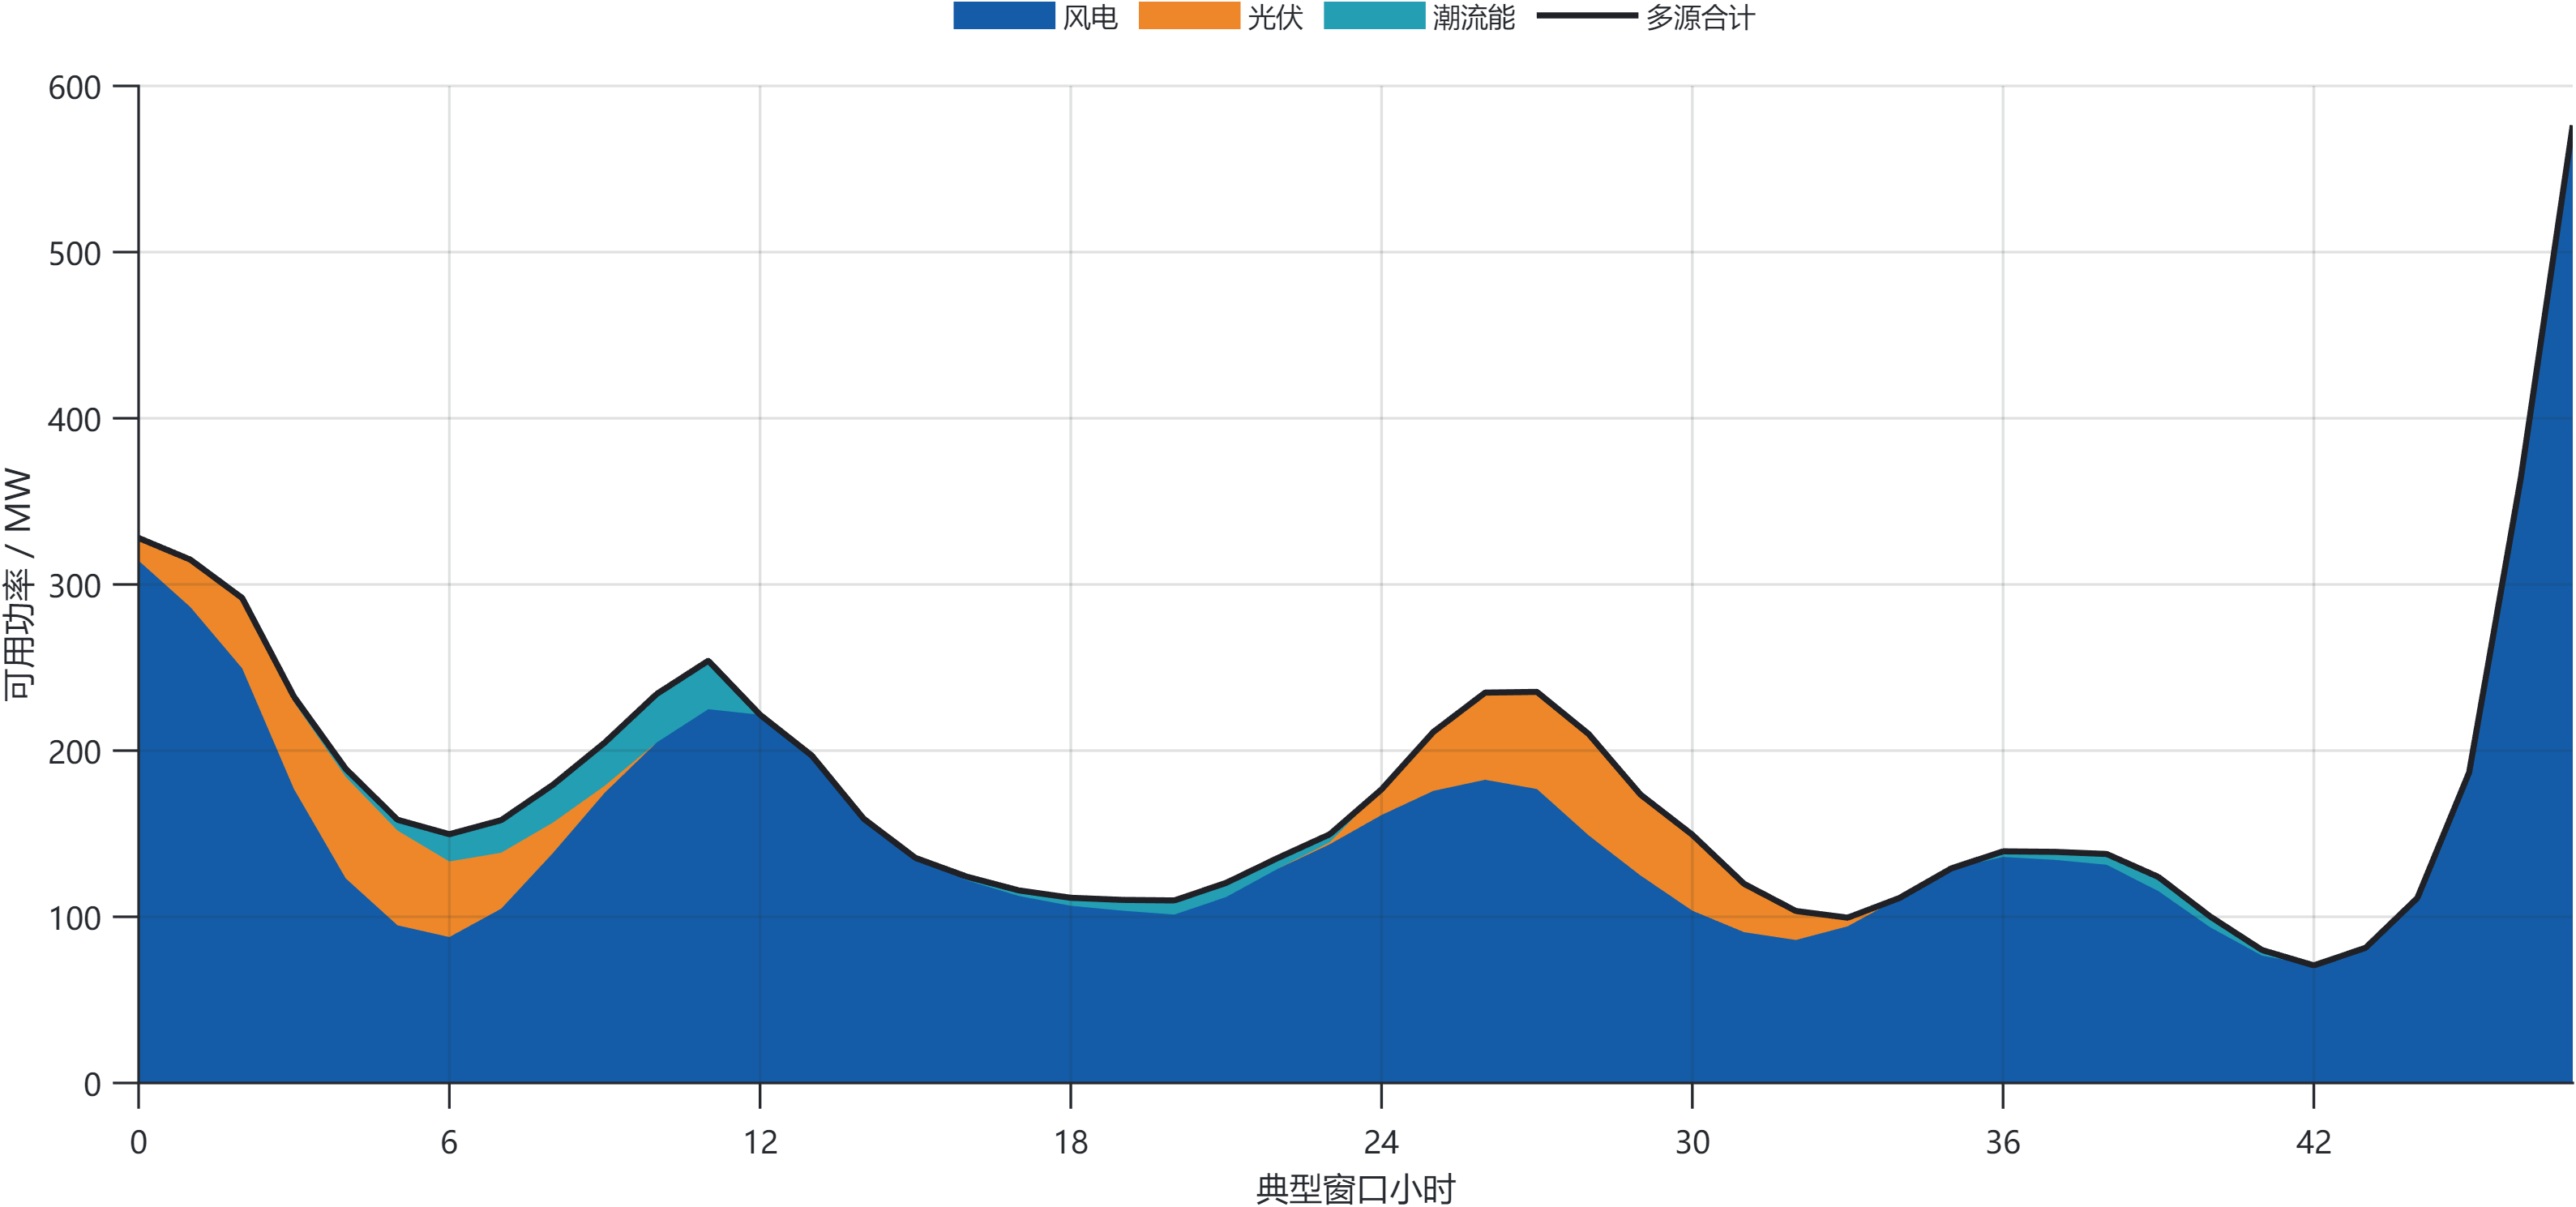
\includegraphics[width=\textwidth]{figures/chapter5/fig5-1_typical48_multisource.png}
\caption{正常典型48 h风、光、潮流多源可用功率}
\label{fig:c5-typical-multisource}
\sourcetype{NASA POWER公开资源代理（政府科研机构公开数据）、项目内部潮流代理
及4.3源侧模型仿真输出；潮流序列为本研究构造。}
\end{figure}

图~\ref{fig:c5-typical-multisource}把表~\ref{tab:c5-typical-source}的总量结果展开为逐时
过程。窗口中风电构成主体，光伏在两个日间时段补充出力，潮流能幅值较小但提供了不同
相位的连续分量；第47小时的总功率陡升主要来自风电代理。该图用于说明本轮比较确实
使用同一条多源逐时曲线及其互补形态，无法据此推断目标海域的资源相关性或极端爬坡概率。

四方案均从BESS 80~MWh、氢库存0~kg开始，全部基础算力为零，海洋刚性需求18~MW，
源侧、价格和PUE逐时输入完全相同。因而表内差异不来自资源窗口或物理初态差异。

\subsection{能量、产品与可靠性结果}

\begin{table}[htbp]
\centering
\caption{正常典型48 h四方案消纳与可靠性结果}
\label{tab:c5-typical-energy}
\begin{tabular}{lrrrr}
\toprule
方案 & 利用/MWh & 弃电/MWh & 消纳率/\% & ENS/MWh\\
\midrule
纯电资产基准 & 7796.323 & 654.475 & 92.255 & 0\\
纯氢资产基准 & 1090.276 & 7360.523 & 12.901 & 0\\
纯算资产基准 & 2317.100 & 6133.699 & 27.419 & 0\\
在线先验--后验 & 7938.057 & 512.742 & 93.933 & 0\\
\bottomrule
\end{tabular}
\end{table}

\begin{table}[htbp]
\centering
\caption{正常典型48 h四方案产品投入与输出结果}
\label{tab:c5-typical-product}
\resizebox{0.95\textwidth}{!}{%
\begin{tabular}{lrrrr}
\toprule
方案 & 海缆受端/MWh & 制氢输入/MWh & 算力输入/MWh & 算力服务/MWh-CS\\
\midrule
纯电资产基准 & 6145.770 & 0 & 0 & 0\\
纯氢资产基准 & 0 & 0 & 0 & 0\\
纯算资产基准 & 0 & 0 & 1226.824 & 1148.243\\
在线先验--后验 & 5368.917 & 0 & 999.070 & 935.063\\
\bottomrule
\end{tabular}}
\end{table}

全部方案ENS为零，说明该正常窗口内共同源侧与BESS足以覆盖内部及海洋刚性负荷。在线
策略实际E/H/C可选输入比例为85.383\%/0\%/14.617\%。相对纯电基准，在线策略消纳率
提高1.677个百分点、弃电减少141.733~MWh；但正如前述，这一差异既来自柔性算力通道，
也来自在线计划，无法归为纯控制算法增益。

\subsection{运行层经济结果}

\begin{table}[htbp]
\centering
\caption{正常典型48 h四方案运行层经济分账}
\label{tab:c5-typical-economics}
\resizebox{0.95\textwidth}{!}{%
\begin{tabular}{lrrrr}
\toprule
方案 & 输出收入/万元 & 可变成本/万元 & 期末调整/万元 & 净收益/万元\\
\midrule
纯电资产基准 & 248.496 & 16.311 & $-2.186$ & 234.371\\
纯氢资产基准 & 25.920 & 2.181 & $-2.186$ & 25.926\\
纯算资产基准 & 83.332 & 4.634 & $-2.186$ & 80.884\\
在线先验--后验 & 266.964 & 16.235 & $-2.186$ & 252.915\\
\bottomrule
\end{tabular}}
\end{table}

运行净收益定义为输出收入减可变运行成本，再扣除期末库存调整的成本口径；它不含CAPEX、
固定运维、替换、折旧、税费、融资、保险、退役和全寿命风险。四方案期末SOC均为0.89375，
高于80~MWh初始电量，按347~CNY/MWh的假设终端价值形成共同$-21,861$~CNY成本调整，
即净收益中的等额存量增值。该处理避免免费占用窗口末电量，但也说明本表并非现金收入表。

在线策略相对纯电基准运行净收益提高185,443~CNY，即7.91\%。该比较在相同短窗口和共同
终端估值下有效，但由于资产组合不对称、且未计新增算力和制氢资产CAPEX，不足以推导投资
回收期、净现值或全寿命收益率。

\begin{figure}[H]
\centering
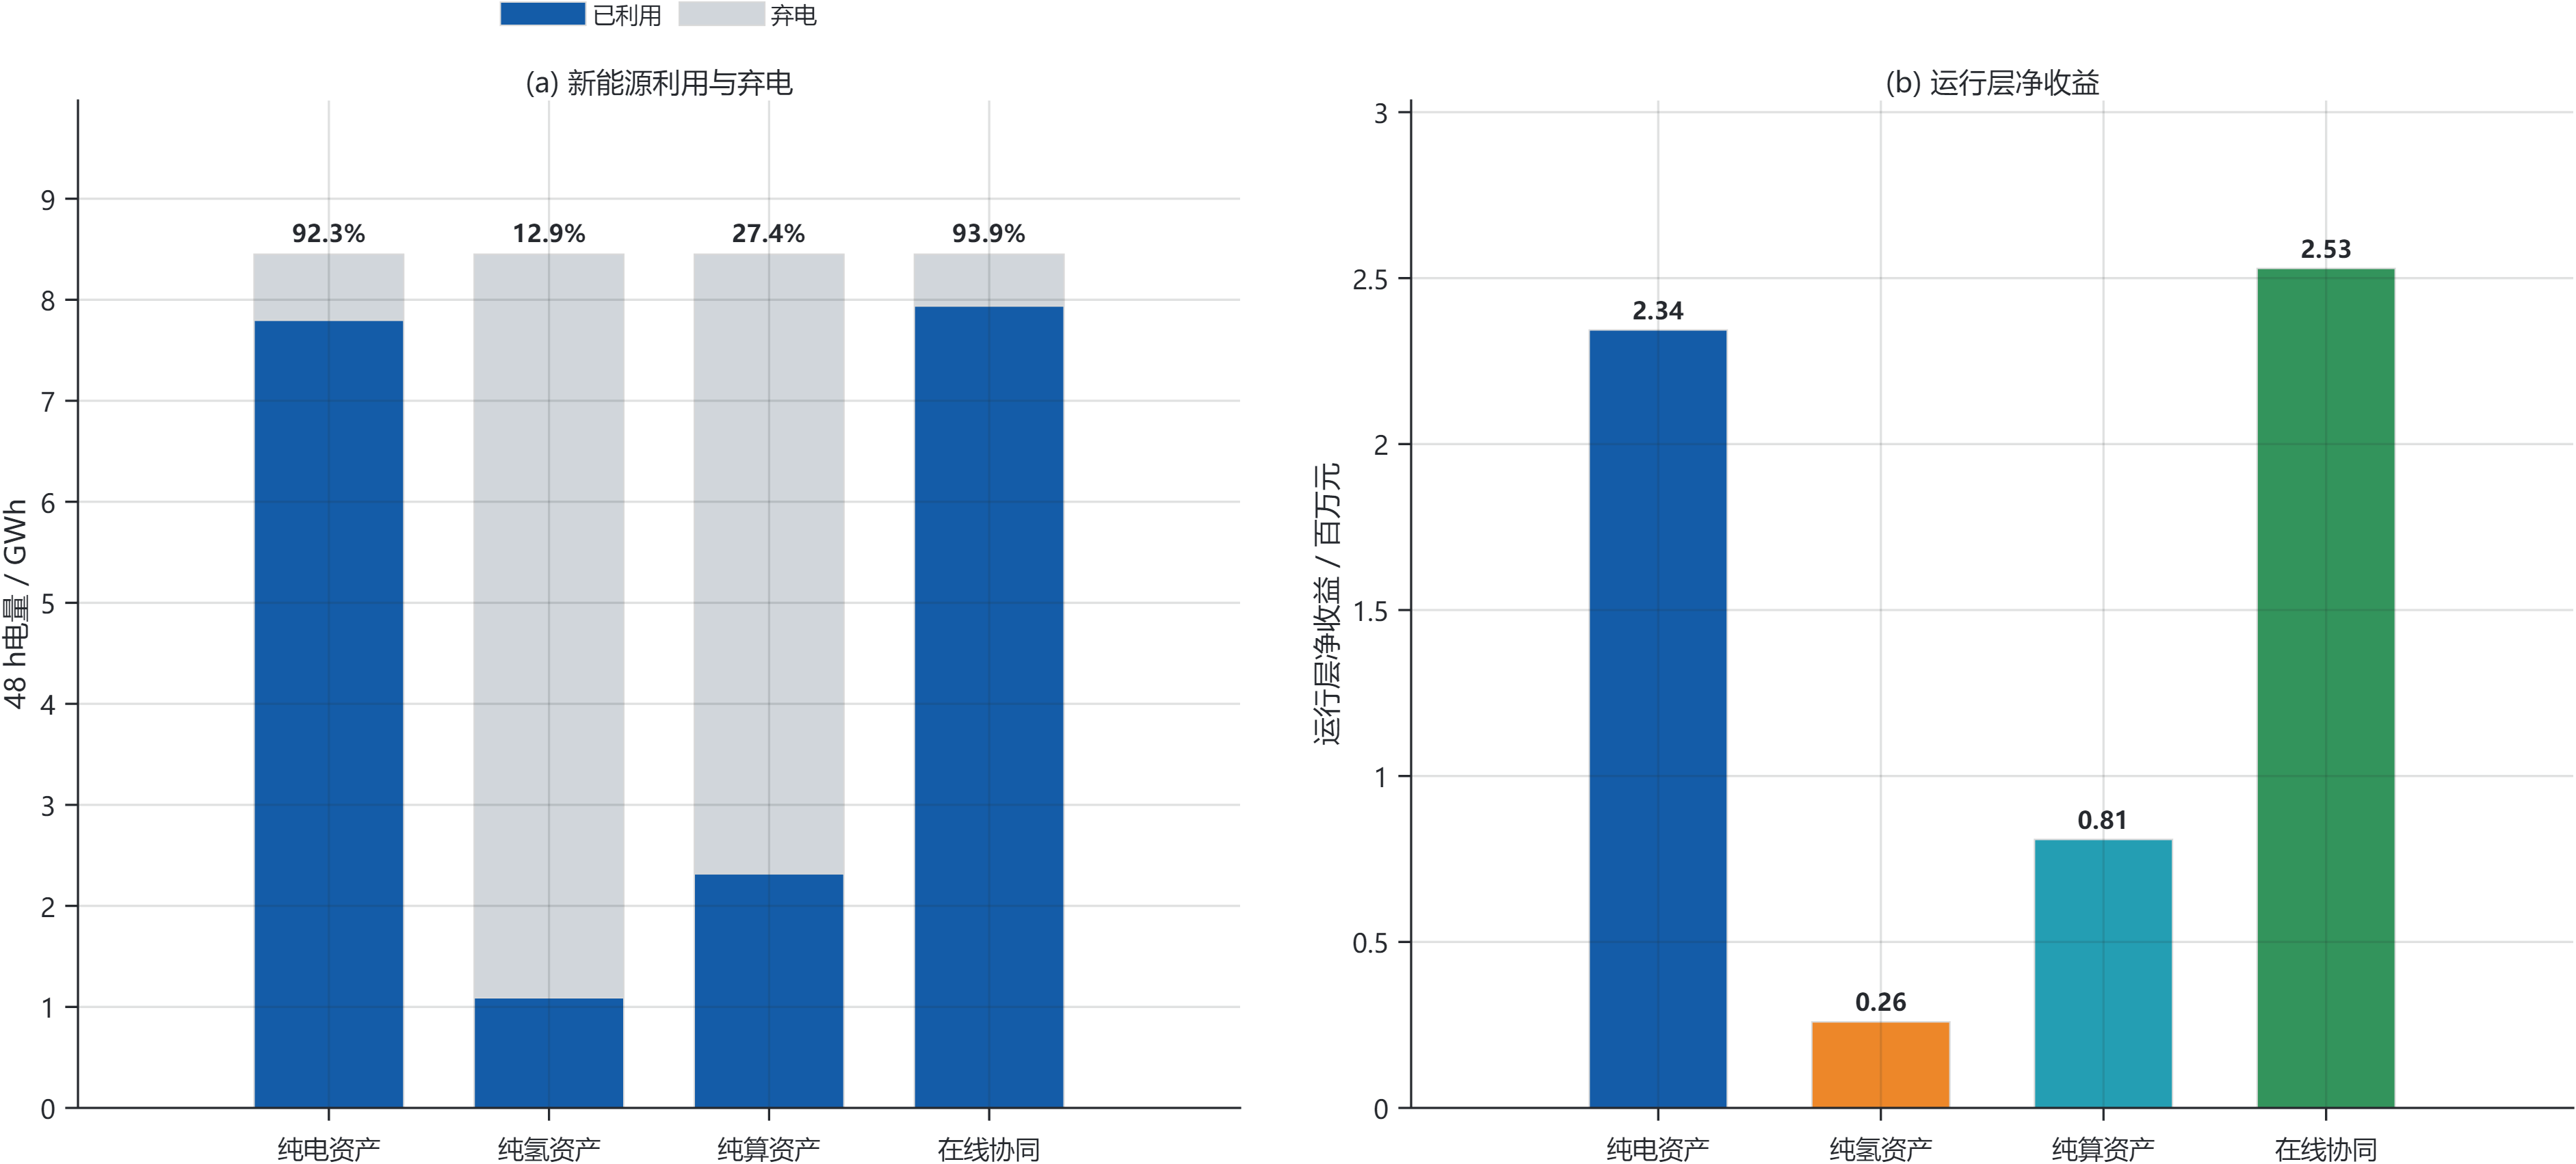
\includegraphics[width=\textwidth]{figures/chapter5/fig5-2_typical48_strategy_comparison.png}
\caption{正常典型48 h四方案新能源利用及运行层净收益比较}
\label{fig:c5-strategy-comparison}
\sourcetype{项目组MATLAB模型仿真输出；设备、价格、惩罚和终端价值参数采用本研究的基准取值。}
\end{figure}

图~\ref{fig:c5-strategy-comparison}左侧同时保留已利用电量和弃电量，避免只报告消纳率；
右侧采用同一运行层净收益口径。在线协同在该窗口的消纳率和净收益均最高，但图中差异是
“产品资产组合+在线计划”的联合结果，其中7.91\%无法拆解为算法单独贡献。纯氢方案的
低利用率也与表~\ref{tab:c5-typical-product}一致：当前价格与零承购约束下模型没有人为制氢。

\subsection{分方案行为解释}

\subsubsection{纯电资产基准}

纯电方案将6.680~GWh送入海缆，受端获得6.146~GWh，差额符合8\%固定损耗。
海缆200~MW上限和BESS有效SOC边界共同限制进一步消纳。其最低时末SOC为0.10625，说明
经济调度曾充分调用BESS；终端又回充至0.89375。该方案是本轮最强单一产品基准，但海缆
损耗率、受端价格和容量采用本研究的基准取值。

\subsubsection{纯氢资产基准}

尽管电解、储氢和相关资产处于启用状态，电解输入、产氢和供应量均为数值零。模型只利用
1,090.276~MWh新能源服务共同刚性负荷并形成期末BESS库存，其余弃电。原因是当前28.36
~CNY/kg氢价、56.77~kWh/kg固定SEC、启动及变动成本、零最低承购和零期末强制氢库存
组合下，在当前价格、设备效率和最低采购量设定下，制氢未进入最优解。该结果表明氢能路径的经济性
对承购价格、产品等级、储运成本和最低采购量较为敏感，需通过真实合同和价格
敏感性寻找启用阈值。

\subsubsection{纯算资产基准}

纯算方案消耗1,226.824~MWh设施电量，完成1,148.243~MWh-CS算力服务，周期等效PUE为1.0684。
其余利用电量用于共同刚性负荷和BESS状态调整。由于算力设施上限120~MW，小于纯电海缆
200~MW上限，单一算力通道在高出力小时更早饱和，导致消纳率仅27.419\%。MWh-CS是聚合
等效服务量，不等同于GPU小时、Token或任务履约量。

\subsubsection{在线先验--后验策略}

在线策略同时形成5,368.917~MWh海缆受端电量和935.063~MWh-CS算力服务，周期等效PUE
为1.0685；制氢仍为零。预测MAE为39.615~MW，逐源标准差和代理均值192.300~MW。平均
计划份额L1小时变化为0.0279，最大L1变化0.1265，最大单通道变化0.0632，死区保持15~h；
48~h内没有计划回退、储备释放或可靠性放宽，实际计划偏差不超过0.15。说明计划平滑和小时
比例约束在正常短窗口按设定生效，但尚未进行概率校准和控制参数优选。

\begin{figure}[H]
\centering
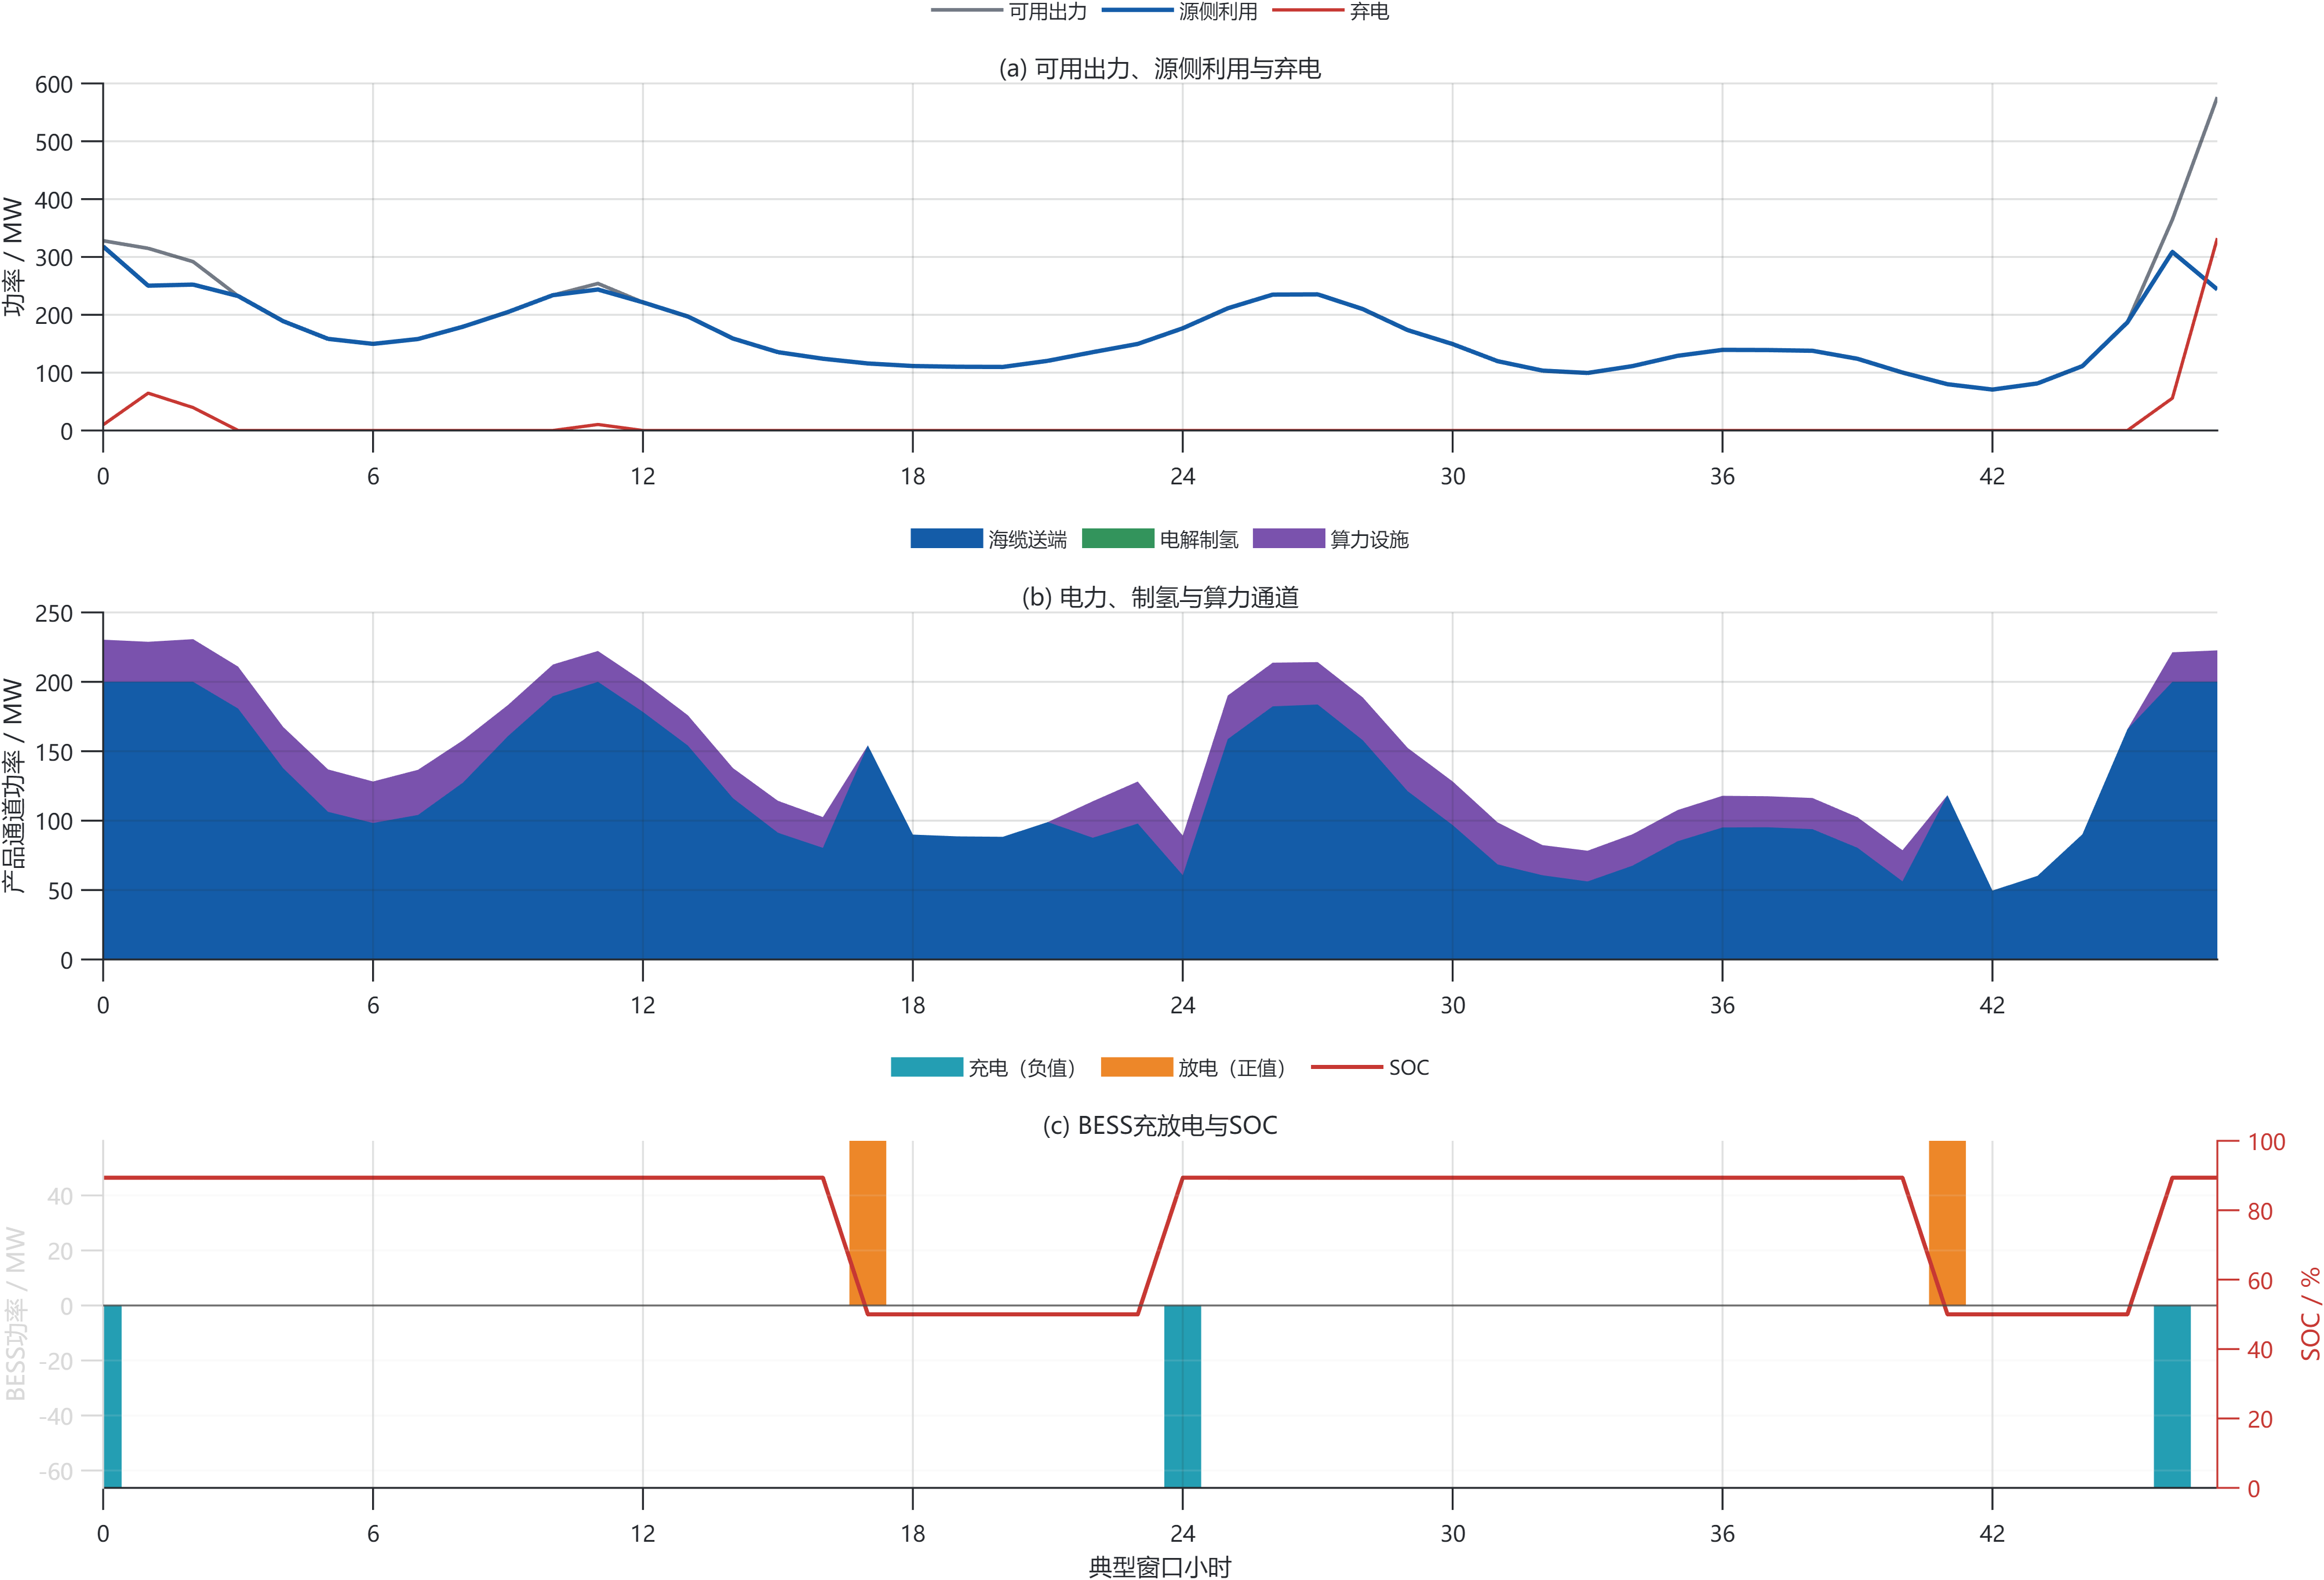
\includegraphics[width=\textwidth]{figures/chapter5/fig5-3_typical48_online_dispatch.png}
\caption{正常典型48 h在线策略源侧利用、产品分配与BESS调度}
\label{fig:c5-online-dispatch}
\sourcetype{项目组MATLAB模型逐时仿真输出；图中功率为1 h步长下的小时平均值。}
\end{figure}

图~\ref{fig:c5-online-dispatch}展示在线策略的物理执行结果。海缆承担主要可选消纳，算力
形成约20--35~MW的补充柔性通道，制氢功率保持为零；BESS仅在源侧突升或产品通道受限
时集中充放电。第47小时可用出力升至576.311~MW，但海缆和算力均接近容量上限，BESS
又执行充电，仍产生明显弃电。该现象说明弃电来自通道容量与小时调度共同约束，而非把
可用发电量预先给定。

\begin{figure}[H]
\centering
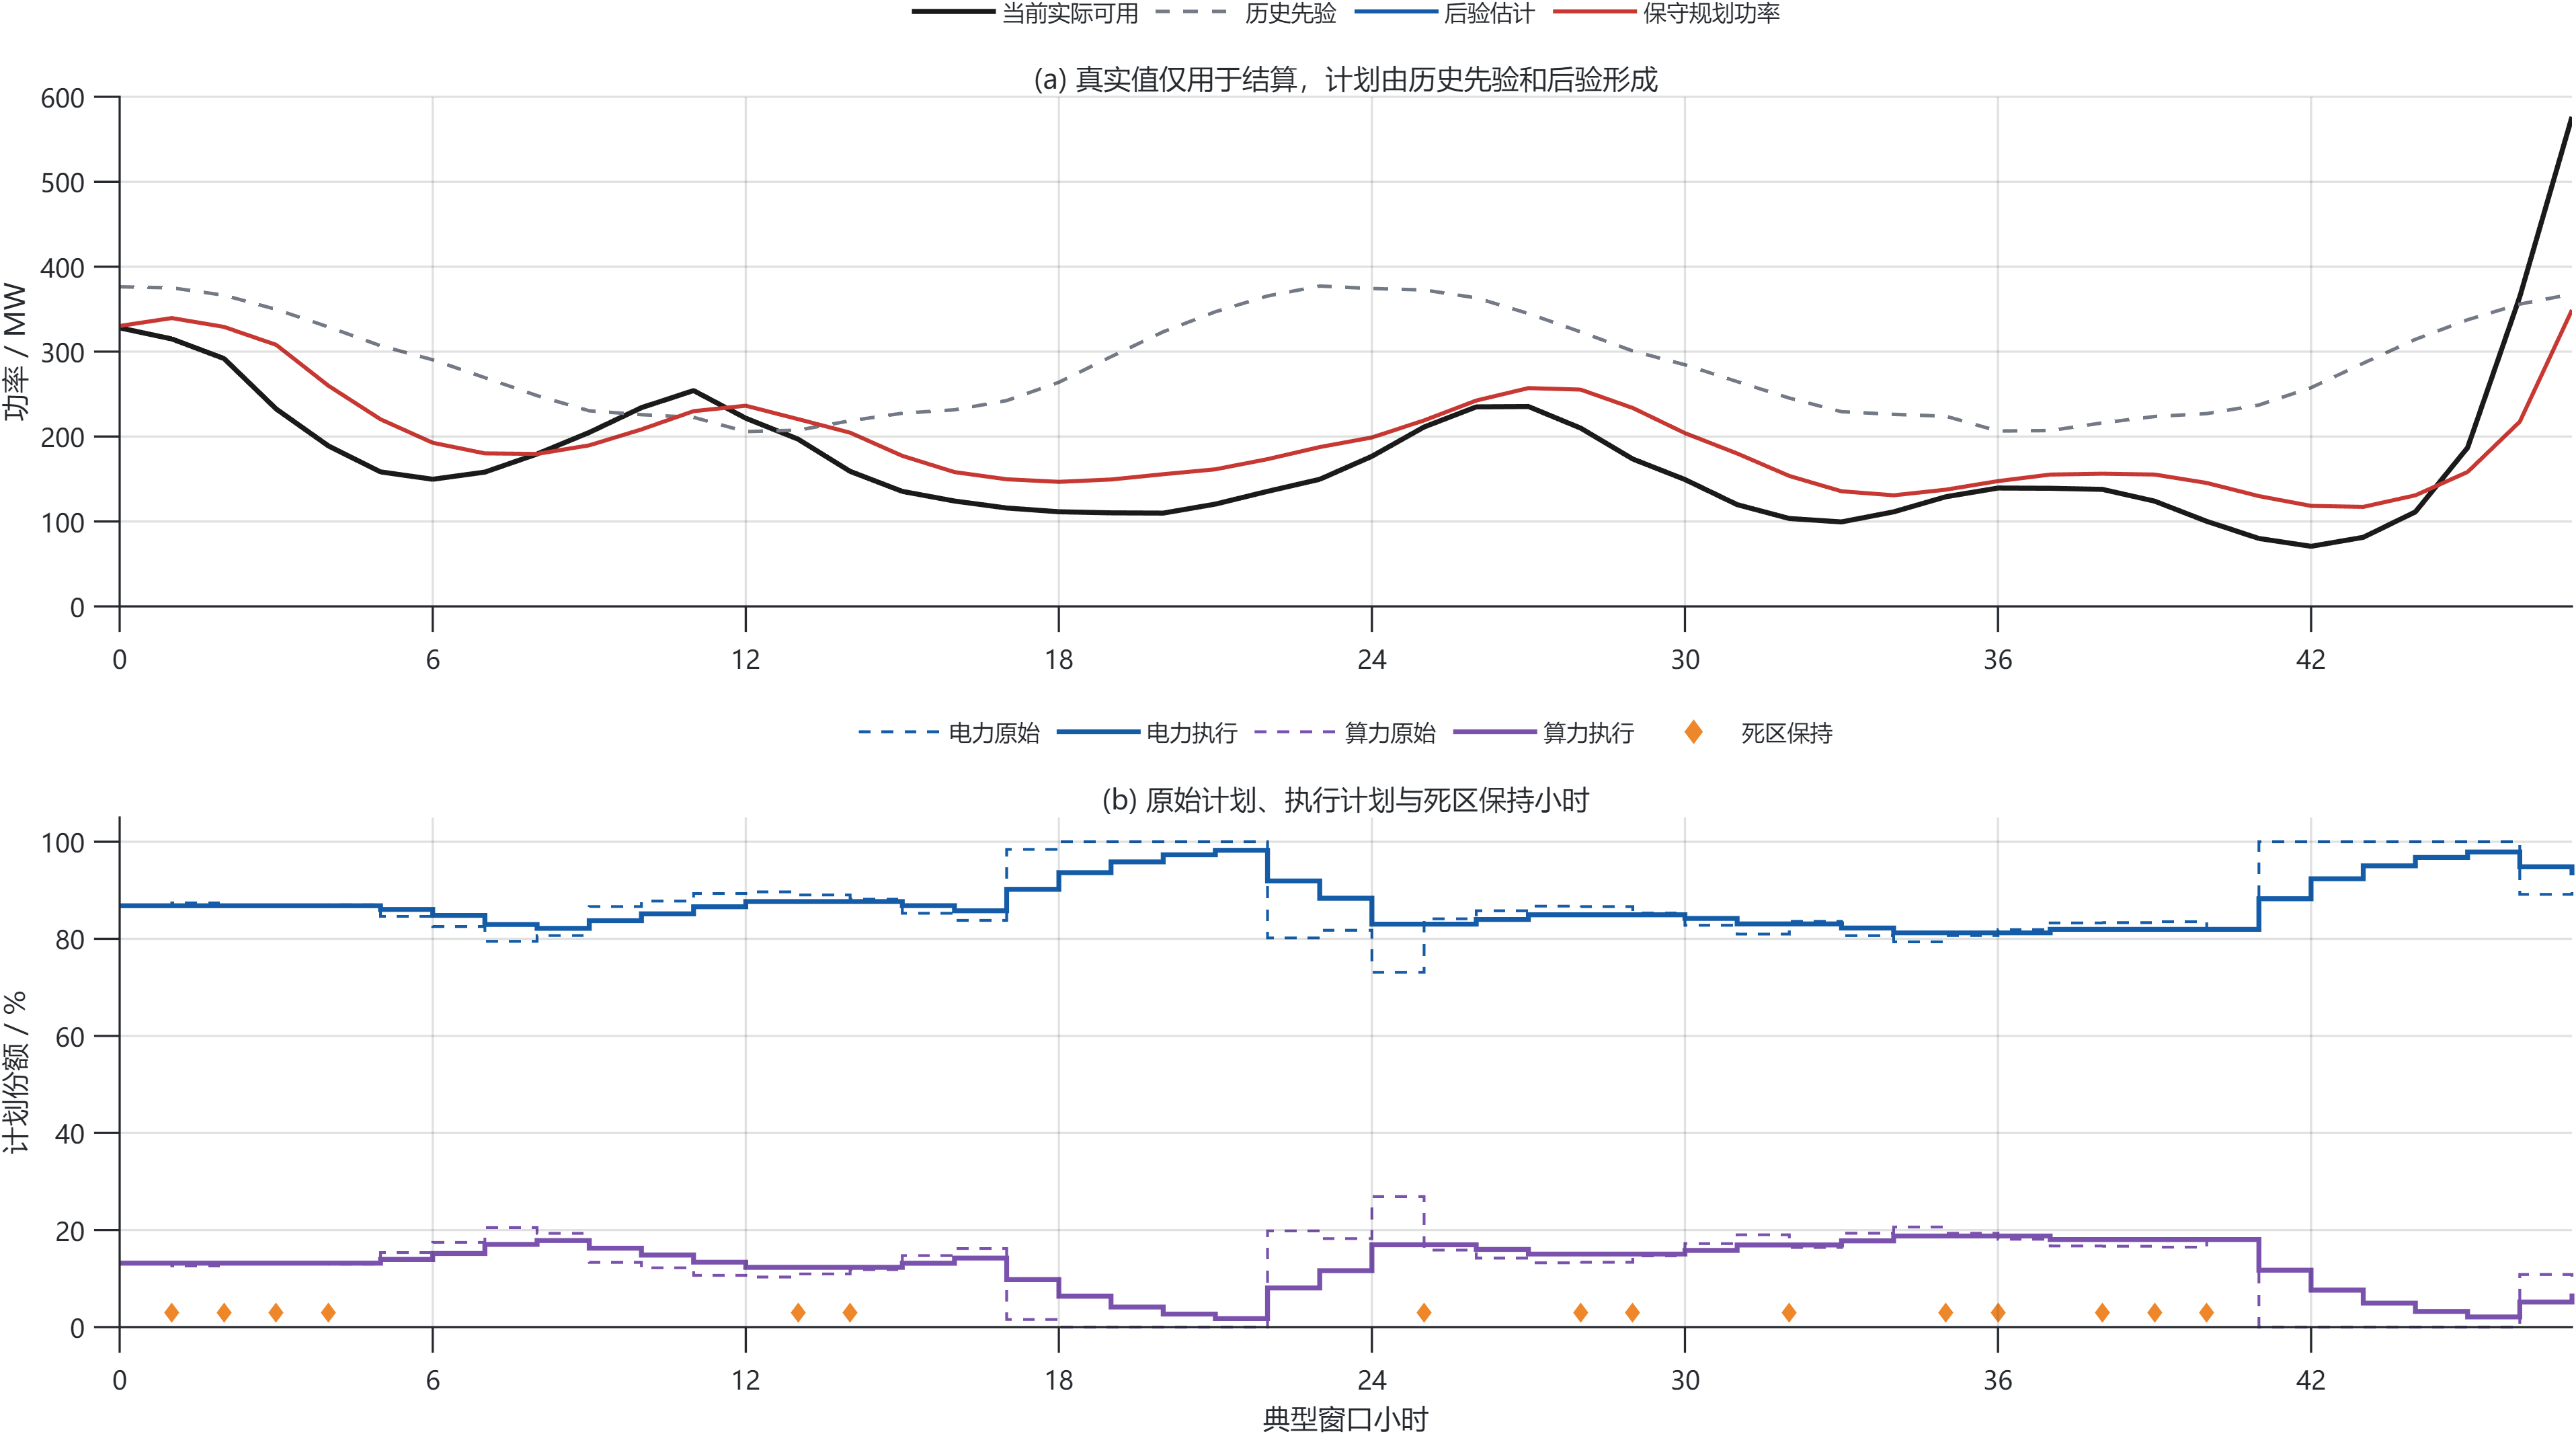
\includegraphics[width=\textwidth]{figures/chapter5/fig5-4_forecast_and_anti_jitter.png}
\caption{正常典型48 h先验--后验功率修正与计划份额计划平滑}
\label{fig:c5-forecast-antijitter}
\sourcetype{项目组MATLAB模型逐时仿真输出；预测与计划平滑参数采用本轮控制试验的基准取值。}
\end{figure}

图~\ref{fig:c5-forecast-antijitter}(a)把当前实际可用功率与历史先验、后验估计和保守规划
功率并列，实际值只在当前小时结算时进入账本，不回写为事前已知量。图
~\ref{fig:c5-forecast-antijitter}(b)进一步对比原始份额和执行份额；橙色菱形所示15个小时
触发死区保持，执行曲线因此没有逐小时追随全部小幅变化。该图能够证明因果信息边界与计划平滑
逻辑按代码执行，但曲线贴近程度无法替代预测区间覆盖率、可靠度图或概率校准检验。

\subsection{运行层环境代理}

按第4章式~\eqref{eq:environment-objective}和当前配置复算表~\ref{tab:c5-typical-env}。
已用新能源和BESS充放吞吐因子分别取15和5~kgCO$_2$e/MWh，电、算和海洋服务基准因子
均取500~kgCO$_2$e/MWh。上述因子用于运行层情景比较，结果不构成ISO
14040/14044产品LCA或认证减排量\cite{iso14040,iso14044}。

\begin{table}[htbp]
\centering
\caption{正常典型48 h运行层温室气体代理}
\label{tab:c5-typical-env}
\resizebox{\textwidth}{!}{%
\begin{tabular}{lrrr}
\toprule
方案 & 项目排放代理/tCO$_2$e & 避免排放代理/tCO$_2$e & 净排放代理/tCO$_2$e\\
\midrule
纯电资产基准 & 119.800 & 3504.885 & $-3385.085$\\
纯氢资产基准 & 16.686 & 432.000 & $-415.314$\\
纯算资产基准 & 35.088 & 1006.122 & $-971.034$\\
在线先验--后验 & 120.664 & 3583.990 & $-3463.326$\\
\bottomrule
\end{tabular}}
\end{table}

负值表示在当前既定基准因子下“避免排放大于项目运行代理排放”，不宜表述为已核证碳减排。
建设、海工、海缆、设备更换、冷媒、船舶航次、氢产品分摊和退役尚未进入清单。

\section{8,760 h年度因果运行与极端事件验证}

\subsection{年度总量与源侧构成}

年度只运行在线先验--后验策略。三源可用新能源合计2,014,114.533~MWh，实际利用
1,294,715.936~MWh，弃电719,398.597~MWh，消纳率64.282\%。小时平均可用功率
229.922~MW，最大743.842~MW；零源侧出力共148~h，其中24~h来自构造的台风过境过程，另有
124~h来自正常阶段资源--功率曲线代理。正常零出力时数较多，是年度可靠性结果需要场址
数据校准的重要信号。

\begin{table}[htbp]
\centering
\caption{年度多源可用新能源构成}
\label{tab:c5-annual-source}
\begin{tabular}{lrr}
\toprule
电源 & 年度可用电量/MWh & 电量占比/\%\\
\midrule
漂浮式风电代理 & 1830468.696 & 90.882\\
漂浮式光伏代理 & 139937.714 & 6.948\\
潮流能代理 & 43708.124 & 2.170\\
合计 & 2014114.533 & 100.000\\
\bottomrule
\end{tabular}
\end{table}

名义容量85\%/10\%/5\%与可用电量90.882\%/6.948\%/2.170\%不同，说明模型没有按
装机比例固定发电量；差异由资源、功率曲线、辅机、损耗和状态共同产生。但由于风高、辐照
分解和潮流输入仍是代理，该电量结构不宜作为工程年发电量结论。

\begin{figure}[H]
\centering
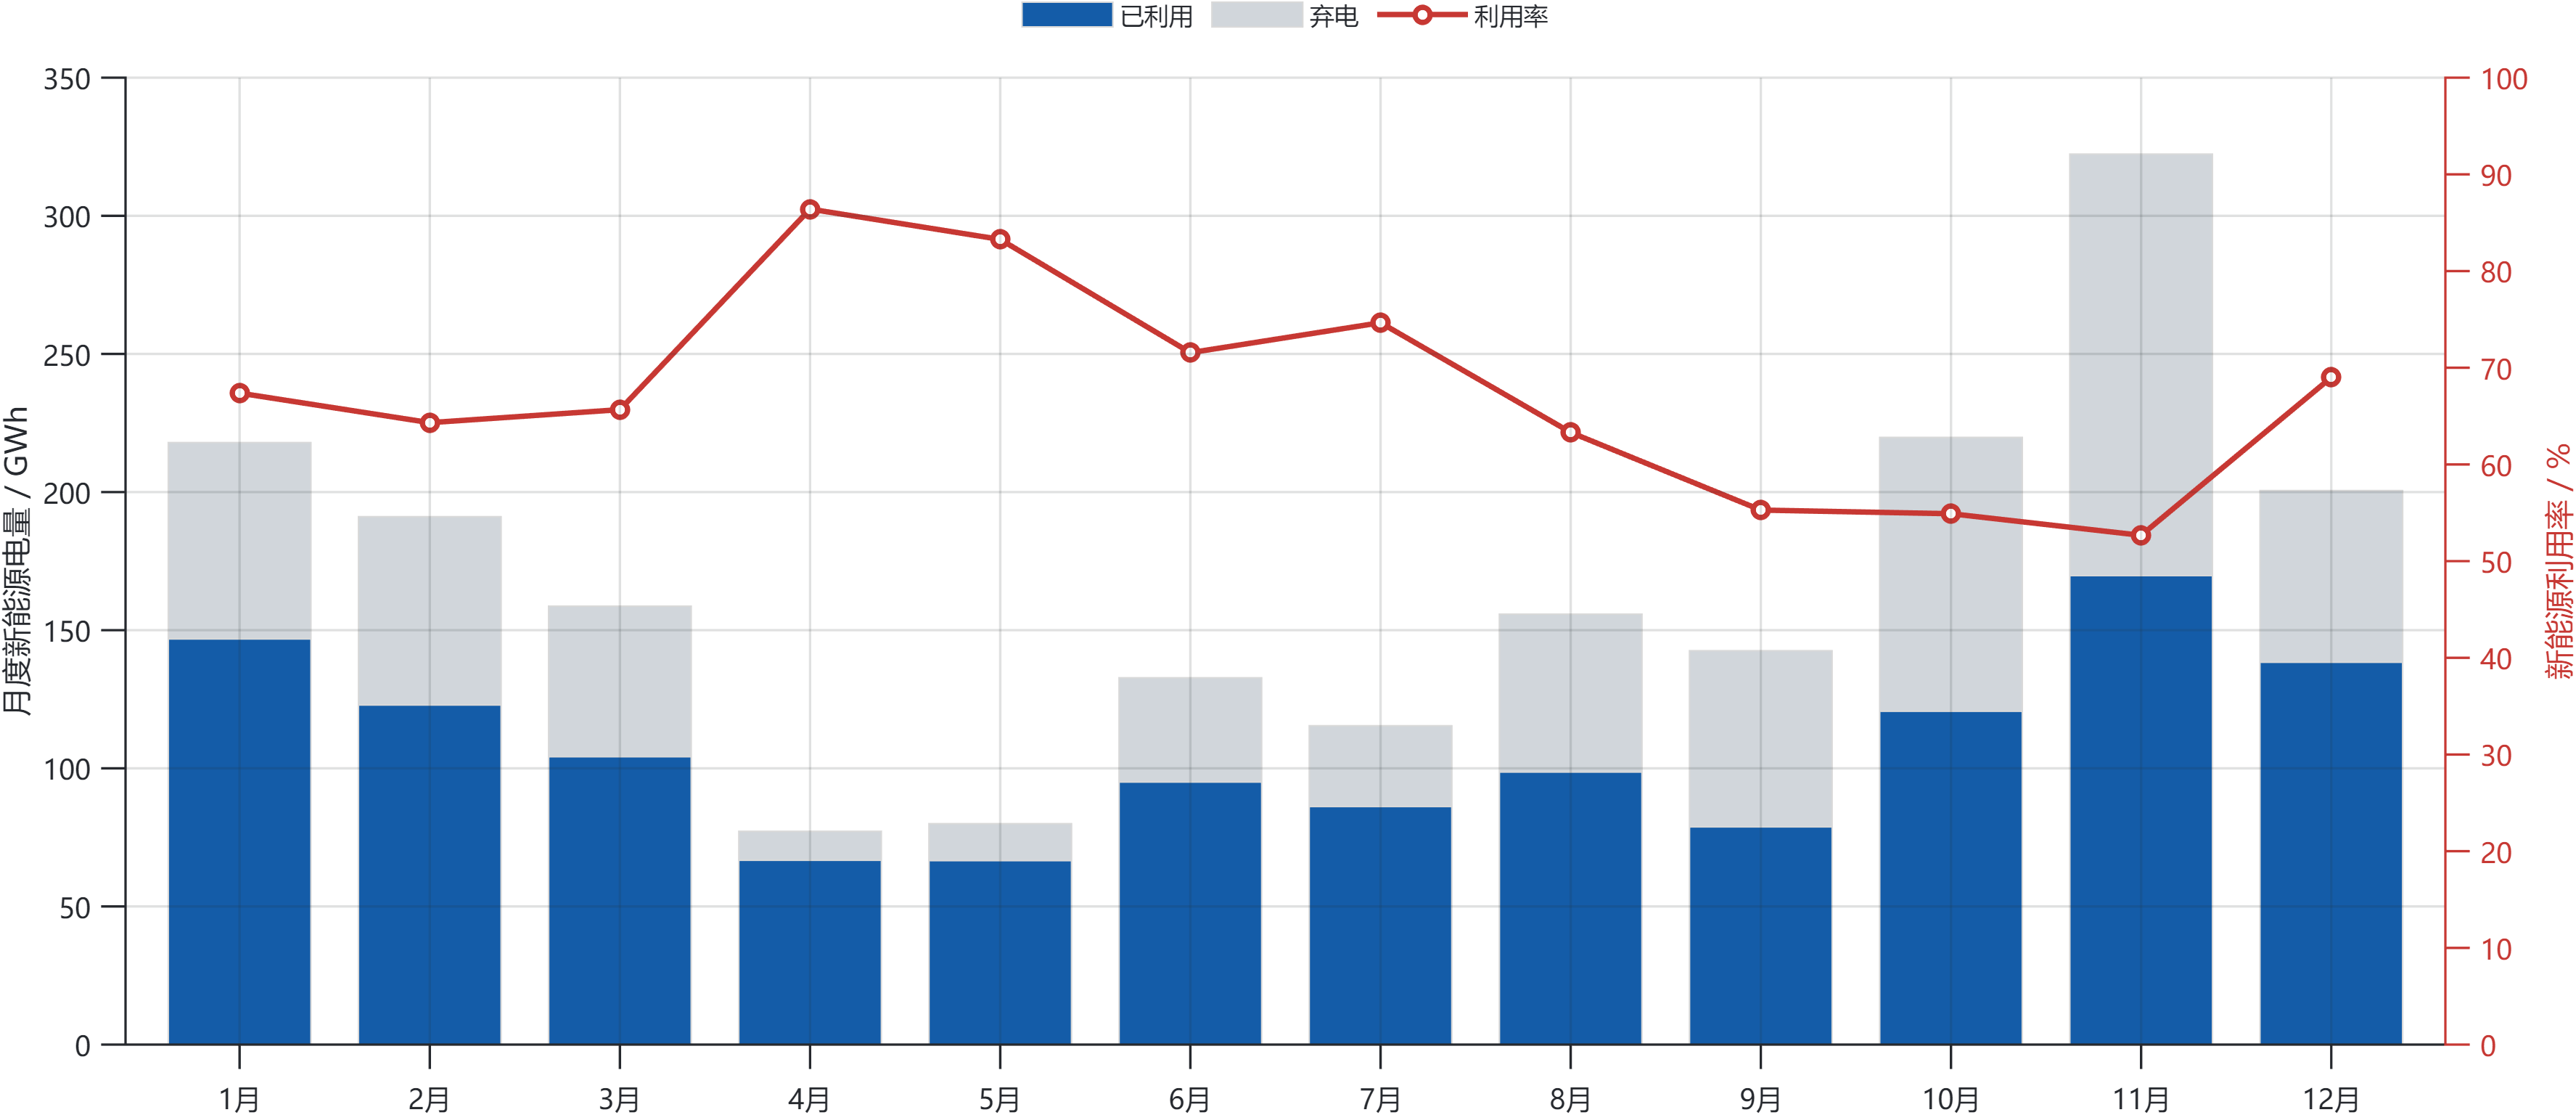
\includegraphics[width=\textwidth]{figures/chapter5/fig5-5_annual_monthly_energy.png}
\caption{年度逐月新能源利用、弃电与利用率}
\label{fig:c5-annual-monthly-energy}
\sourcetype{项目组MATLAB模型8760 h仿真输出；资源代理和设备参数的证据状态同
第5.1节。}
\end{figure}

图~\ref{fig:c5-annual-monthly-energy}显示64.282\%的年度利用率并非各月均匀结果。4--5月
可用电量较低但利用率超过80\%，而9--11月利用率约处于50\%--56\%区间；11月可用电量
最高，同时弃电也最大。由此可见，当前主要矛盾不只是“年发电量不足”，还包括高资源月份
产品通道和储能容量不足。上述月份特征仍受NASA资源代理、风高处理及重复潮流序列影响，
需在场址实测或再分析数据校准后再用于容量规划。

\subsection{产品分配与服务结果}

\begin{table}[htbp]
\centering
\caption{年度在线策略核心结果}
\label{tab:c5-annual-summary}
\resizebox{0.94\textwidth}{!}{%
\begin{tabular}{lr@{\qquad}lr}
\toprule
指标 & 结果 & 指标 & 结果\\
\midrule
可用新能源 & 2014114.533~MWh & 利用新能源 & 1294715.936~MWh\\
弃电量 & 719398.597~MWh & 消纳率 & 64.282\%\\
海缆送端输入 & 945433.733~MWh & 海缆受端电量 & 869799.034~MWh\\
柔性算力输入 & 167339.049~MWh & 算力服务 & 155760.730~MWh-CS\\
制氢输入/氢气供应 & 0/0 & 周期等效PUE & 1.0743\\
ENS & 7128.526~MWh & 关键负荷服务率 & 96.184\%\\
输出收入 & 453.614百万元 & 运行净收益 & 342.111百万元\\
\bottomrule
\end{tabular}}
\end{table}

年度实际E/H/C可选投入比例为84.962\%/0\%/15.038\%。制氢输入、氢库存、氢气供应和
氢转电均为数值零。虽然配置中启用30~MW氢转电额定容量，但年度没有自然形成氢库存，
因此该支路没有提供任何韧性。当前基本场景实际验证的是“电力+算力”组合，而非三产品
均被激活；项目陈述需把“氢路径具备架构接口”与“氢价值已被年度结果证明”分开。

\subsection{可靠性分解}

年度关键需求总量186,782.640~MWh，其中内部关键需求29,102.640~MWh、海洋刚性需求
157,680.000~MWh、基础算力需求0。ENS按负荷分解见表~\ref{tab:c5-annual-reliability}。

\begin{table}[htbp]
\centering
\caption{年度ENS及服务率分解}
\label{tab:c5-annual-reliability}
\begin{tabular}{lrrr}
\toprule
负荷类别 & 需求/MWh & ENS/MWh & 服务率/\%\\
\midrule
内部关键负荷 & 29102.640 & 342.209 & 98.824\\
海洋刚性负荷 & 157680.000 & 6786.317 & 95.696\\
基础算力负荷 & 0 & 0 & 不适用\\
合计 & 186782.640 & 7128.526 & 96.184\\
\bottomrule
\end{tabular}
\end{table}

海洋刚性负荷贡献95.199\%的年度ENS，是可靠性短板的主要来源；内部关键负荷仅由现有
辅机和固定损失字段构成，尚不代表完整能源岛关键负荷清单。算力服务率无法从该表推导，
因为本轮算力全部可中断，未执行部分并非ENS。

\begin{figure}[H]
\centering
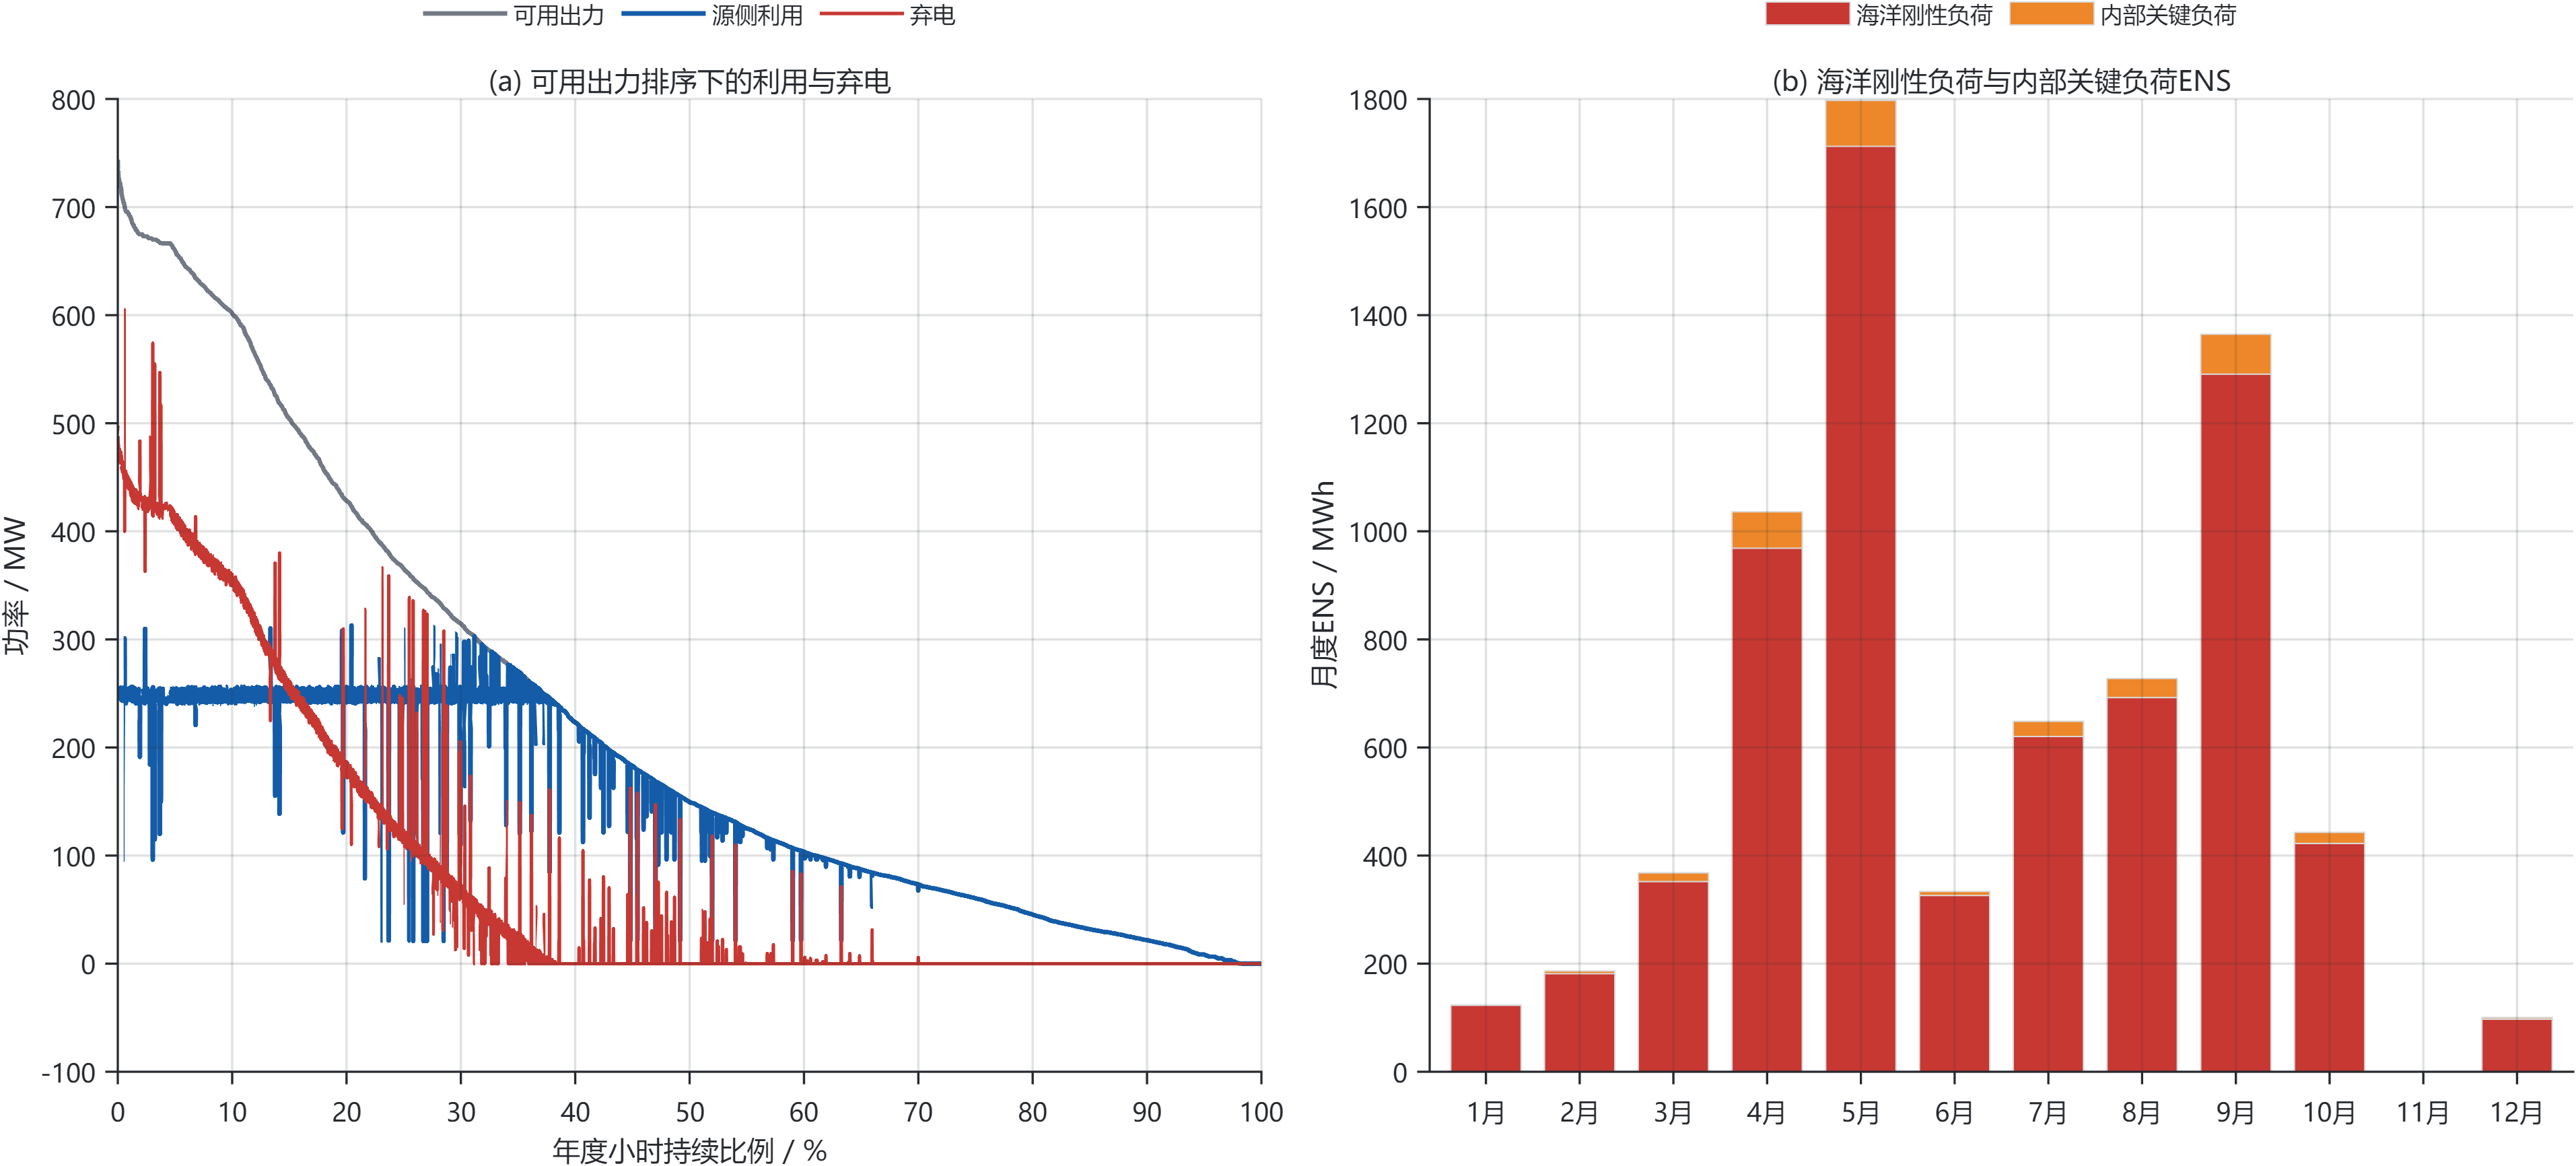
\includegraphics[width=\textwidth]{figures/chapter5/fig5-6_annual_duration_and_ens.png}
\caption{年度出力持续曲线与月度ENS构成}
\label{fig:c5-duration-ens}
\sourcetype{项目组MATLAB模型8760 h逐时仿真输出。}
\end{figure}

图~\ref{fig:c5-duration-ens}(a)按可用出力从高到低排列年度小时，显示高出力区间的已利用
功率长期受海缆、算力和储能容量约束，弃电主要集中在持续曲线前段；低出力区间则逐步转化
为可靠性问题。图~\ref{fig:c5-duration-ens}(b)表明月度ENS以海洋刚性负荷为主，4、5、7、
8和9月较为突出，11月则为零。该分布再次说明年度ENS主要来自正常低出力时段，并非只在
人为台风事件中产生；同时也提示应分别研究扩容消纳设备和补充长时保供资源，不宜采用同一
设备同时解决全部高出力弃电与长时间低出力缺供。

\subsection{预警--过境--恢复分相结果}

\begin{table}[htbp]
\centering
\caption{年度极端事件分相结果}
\label{tab:c5-event-result}
\resizebox{\textwidth}{!}{%
\begin{tabular}{lrrrrrrrr}
\toprule
阶段 & 时长/h & 可用/MWh & 利用/MWh & 弃电/MWh & ENS/MWh & 服务率/\% & 最低SOC & 储备/可靠性释放h\\
\midrule
正常 & 8700 & 2005898.940 & 1292391.473 & 713507.467 & 6770.978 & 96.351 & 0.10625 & 1105/525\\
预警 & 12 & 1473.472 & 374.121 & 1099.352 & 0 & 100.000 & 0.40787 & 2/0\\
过境 & 24 & 0 & 0 & 0 & 341.340 & 25.963 & 0.10625 & 18/18\\
恢复 & 24 & 6742.121 & 1950.343 & 4791.778 & 16.209 & 96.815 & 0.10625 & 2/1\\
\bottomrule
\end{tabular}}
\end{table}

预警开始前一小时末SOC约0.204，首个预警小时暂停可选产品后回充至0.408，预警末达到
0.89375，说明风险状态机确实促成储备回升。预警阶段仍弃电1,099.352~MWh，是因为可选
产品被暂停且BESS很快达到含向下构网裕度的有效上界；该弃电是韧性换消纳的显式代价。

过境期连续24~h源侧为零。BESS从0.89375降至0.10625，可释放储能为
\begin{equation}
\begin{aligned}
E^{usable}&=160(0.89375-0.10625)=126.00\ \mathrm{MWh},\\
E^{served}&=126.00\times0.95=119.70\ \mathrm{MWh}.
\end{aligned}
\label{eq:c5-passage-energy}
\end{equation}
式~\eqref{eq:c5-passage-energy}是第4章BESS状态与效率公式的场景代入。过境关键需求为
461.04~MWh，故最小可行ENS为$461.04-119.70=341.34$~MWh，与逐时结果一致。按平均
19.21~MW关键负荷折算，BESS只能覆盖约6.23个等效小时，不足以支撑24~h零出力。恢复首
小时仍出现16.209~MWh ENS，随后资源和储备逐步恢复。

更重要的是，年度总ENS的94.984\%发生在正常阶段，只有4.789\%发生在过境、0.227\%
发生在恢复。由此可知，当前可靠性不足无法只归因于台风；正常资源代理中的连续低出力、
18~MW海洋刚性负荷、1~h短视控制和BESS容量共同造成更大影响。

\begin{figure}[H]
\centering
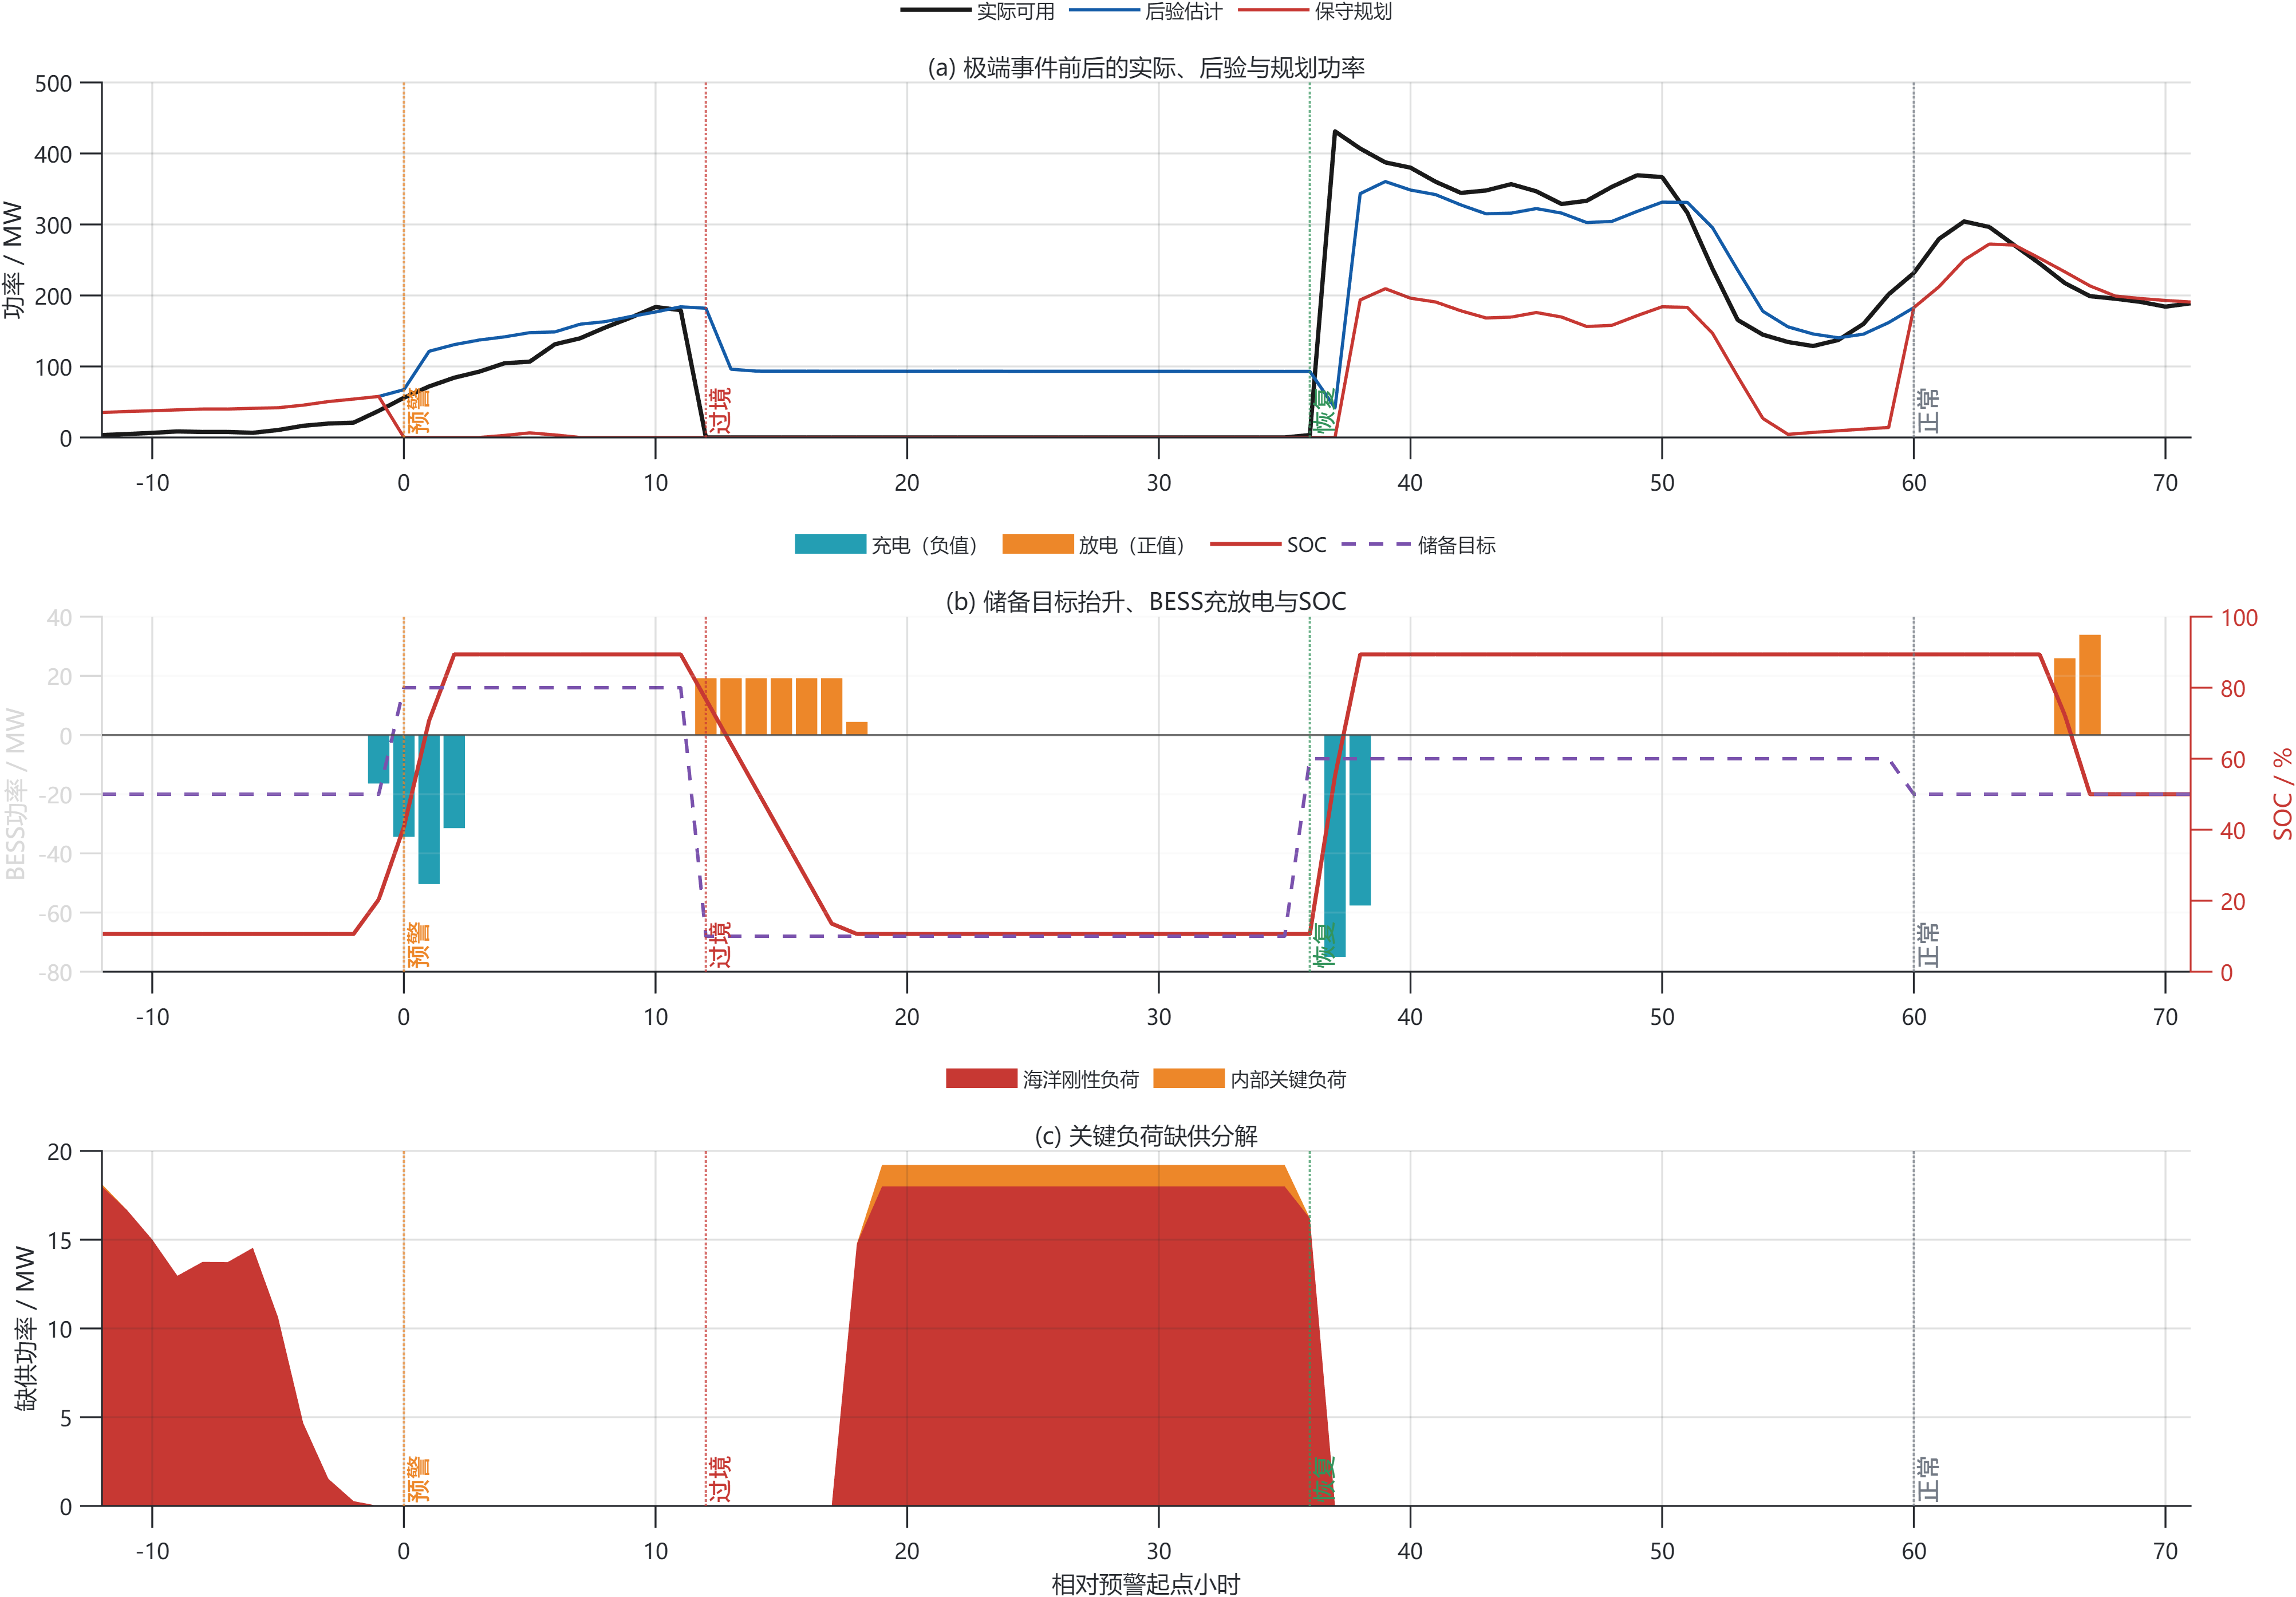
\includegraphics[width=\textwidth]{figures/chapter5/fig5-7_typhoon_response.png}
\caption{台风压力测试中的后验修正、储备响应与关键负荷缺供}
\label{fig:c5-typhoon-response}
\sourcetype{项目组MATLAB模型逐时仿真输出；台风日期、停机、恢复与通道可用率用于构造压力测试过程，不对应历史事件复盘。}
\end{figure}

图~\ref{fig:c5-typhoon-response}把预警前12~h、预警12~h、过境24~h、恢复24~h和恢复后
12~h连续展示。预警开始后保守规划功率迅速收缩，储备目标由正常值抬高至0.8，BESS充电
并达到有效SOC上界；过境阶段源侧和可选产品关闭，BESS持续放电后触及有效下界，关键
负荷缺供随之出现；恢复阶段源侧回归并重新充电。图中预警前仍存在正常阶段ENS，与年度
“正常阶段贡献94.984\% ENS”的统计一致，不应把所有缺供都归因于台风。该响应只证明
小时级能量与状态机逻辑，无法替代平台抗台风、构网动态、黑启动或通信恢复验证。

\subsection{年度运行层经济分账}

\begin{table}[htbp]
\centering
\caption{年度在线策略收入与可变运行成本}
\label{tab:c5-annual-economics}
\begin{tabular}{lrr}
\toprule
项目 & 金额/CNY & 占对应总额/\%\\
\midrule
电力受端收入 & 330465818 & 72.853（收入）\\
算力服务收入 & 77880365 & 17.169（收入）\\
海洋服务价值 & 45268105 & 9.978（收入）\\
输出收入合计 & 453614287 & 100.000\\
\midrule
源侧变动运维 & 25894319 & 23.223（成本）\\
BESS放电退化代理 & 635649 & 0.570（成本）\\
内部ENS惩罚 & 17110470 & 15.345（成本）\\
海洋ENS惩罚 & 67863168 & 60.862（成本）\\
可变运行成本合计 & 111503607 & 100.000\\
\midrule
运行净收益 & 342110681 & ---\\
\bottomrule
\end{tabular}
\end{table}

ENS惩罚合计84.974百万元，占可变运行成本76.207\%，对结果影响显著。50,000~CNY/MWh
内部缺供惩罚和10,000~CNY/MWh海洋缺供惩罚为优化排序参数；在没有服务合同和
违约条款前，它们是优化排序参数，不一定是实际现金支出。年度运行净收益不含CAPEX、固定
运维、人员与船舶、保险、税费、融资、设备替换及退役，不宜解释为净现值、利润或回收期。

\subsection{年度运行层环境代理}

按当前第4章环境代理复算，项目运行排放为19.644~ktCO$_2$e，冻结基准避免排放为
588.227~ktCO$_2$e。两者相减得到净排放代理$-568.583$~ktCO$_2$e。结果主要由
500~kgCO$_2$e/MWh
的电力、算力和海洋服务统一替代因子驱动，相关因子用于本轮情景比较。制氢为零，故本轮没有
绿氢替代减排。该数值不应作为核证自愿减排、绿证、产品碳足迹或ESG披露；需补齐建设、
海缆、平台、储能更换、数据中心设备、船舶、冷媒和退役清单后按ISO 14040/14044重算。

\subsection{预测、控制和求解审计}

年度8,760/8,760~h均返回最优解并通过独立数值审计。544个可靠性放宽小时与544个最小ENS
小时一一对应，实际ENS相对最小可行ENS最大偏差$9.8\times10^{-7}$~MWh；BESS状态递推
最大残差$2.0\times10^{-13}$~MWh。计划份额、SOC储备和可靠性层级分别释放117、1127
和544~h；年度期末SOC回到0.50，最低/最高SOC为0.10625/0.89375，氢库存始终为数值零。

预测MAE为41.047~MW；逐源标准差和代理均值195.156~MW。平均计划份额L1小时变化
0.0423，最大L1变化0.20，最大单通道小时变化0.10；恢复期单通道上限0.05；死区保持
3,608~h。结果说明计划平滑约束按代码设定执行，但并不证明预测分布已经校准。最大BESS储备
短缺79~MWh反映储备目标在可靠性优先时被释放，并非物理SOC越界。

严格零ENS试算每小时使用有限求解时间；最终所有放宽小时又独立求得最小ENS并在容差内
优化经济目标，且结果与逐时缺口一致，因此本轮没有发现因试算超时造成的虚假ENS。但在
更大多时段MILP中仍应区分“证明不可行”和“未在时限内证明”，并保存求解器界与间隙。

\section{合理性、矛盾与异常的完整审查}

\subsection{已消除的前后口径矛盾}

本轮检查已完成以下文档与实现修正：
\begin{enumerate}[label=(\arabic*)]
\item 删除活动文档中22种固定E/H/C比例方案及旧年度三基准结论，统一为“三基准+一在线
      策略”的正常典型48~h比较，年度只验证在线策略；
\item 将第4章联合调度约束由全周期比例改为逐小时因果计划约束，容差统一为0.15，不再使用
      预先已知全期供电量或最低投入；
\item 明确第四章详细算力、规划级海缆损耗和氢放散模型与本章实际采用的聚合接口的差异；
\item 修正年度场景代码中“保留基础算力”的旧注释：当前主场景已将算力全部转为可中断
      柔性容量，基础算力ENS为零；
\item 将年度NASA POWER多源文件补入公开数据清单，并明确50~m风速与GHI处理限制；
\item 将`forecastSigmaMW`改称逐源标准差之和代理，停止称其为聚合预测标准差。
\end{enumerate}

\subsection{仍存在但可以解释的模型现象}

\begin{longtable}{p{2.8cm}p{4.4cm}p{6.1cm}}
\caption{第四章模型与第五章测试的异常审查结论}\label{tab:c5-anomaly-audit}\\
\toprule
现象 & 判断 & 合理解释与后续处理\\
\midrule
\endfirsthead
\toprule
现象 & 判断 & 合理解释与后续处理\\
\midrule
\endhead
年度氢产量和氢转电为零 & 结果合理，但削弱项目氢价值论证 & 当前价格、固定SEC、无最低承购、零氢初态和经济目标共同导致；不应强制造氢，应做承购/价格/效率/长时储能敏感性\\
纯氢基准几乎退化为共同负荷+BESS & 结果由当前价格、效率和最低采购量共同决定 & 需使用真实合同最低量和情景价格识别氢能路径的启用阈值\\
在线策略优于纯电7.91\% & 可作为当前组合效果，无法称纯算法增益 & 新策略拥有算力和氢资产；增加“全资产+当前观测规则”才能隔离算法贡献\\
年度无三基准比较 & 符合本轮范围 & 不应报告年度相对提升；需要时另行统一边界复算\\
94.984\% ENS在正常阶段 & 真实模型信号，并非事件统计矛盾 & 检查正常零出力124~h、海洋刚性负荷、BESS容量、预测与单步控制；工程结论前需校准\\
过境24~h仅服务25.963\% & 与能量边界一致 & 160~MWh BESS可供电119.7~MWh，无法覆盖461.04~MWh需求；须配置长时储能、自然氢库存或负荷分级\\
过境期BESS/储氢仍可用 & 生存性条件尚未验证 & 增加共因故障、生存性、通信中断、辅机耗能和可用率敏感性\\
年度基础算力ENS为零 & 由场景定义，不代表算力可靠 & 全部任务可中断；需另设不可中断SLA、队列和逾期场景\\
内部关键负荷仅约3.32~MW平均 & 边界不完整 & 当前主要为源侧辅机、0.25~MW公共辅机和0.20~MW固定损失；应补完整岛用电清单\\
海缆损耗固定8\% & 可用于统一比较，不宜采用于工程定案 & 按距离、电压、拓扑、换流站与负载率建立设计级损耗或PWL模型\\
WS50M直入155~m风机曲线 & 数据映射尚未验证 & 用测风/再分析多高度数据校准风切变、空气密度、尾流和极端风状态\\
GHI作DHI且DNI为零 & 辐照分解尚未验证 & 使用经验证的辐照分解、组件姿态、海面反照率与热模型\\
潮流能重复48~h & 内部构造的周期性输入 & 用目标海域流速矢量、潮汐调和和波流耦合数据替换\\
典型窗口物理状态重置 & 适合受控比较，并非自然运营 & 另报从年度轨迹继承状态的滚动样本；跨年度验证时避免选择偏差\\
年度仅设置一次台风压力测试 & 只能验证状态机，无法估计概率可靠性 & 建立多强度、多持续时间、多路径、多共因故障场景及概率，届时才能计算EENS\\
单小时在线计划 & 因果但可能短视 & 扩展6/24/48~h滚动MPC，使用当时可获得预报且只执行首时段\\
环境结果大幅为负 & 由既定替代因子驱动 & 仅作运行代理；补全LCA清单、基准、附加性和多产品分摊\\
运行净收益为正 & 仅代表假设运行边际 & 补CAPEX、固定O\&M、税费、融资、替换、保险及退役后再算NPV/FIRR\\
小时审计全部通过 & 证明代数闭合，不证明动态稳定 & 继续REGFM、EMT、HIL、黑启动和现场验收，不应直接声称构网认证\\
\bottomrule
\end{longtable}

综合判断是：本轮未发现能量凭空产生、场外补SOC/补氢、用未来真实出力制定计划、弃电与
关键ENS同小时并存、状态重置、容量越界或结果账本不闭合等硬矛盾。主要问题集中在数据与
场景代表性、资产组合公平性、可靠性配置、详细模块未嵌入、经济/LCA边界不完整，而非
求解器输出自相矛盾。

\section{敏感性设计与下一步验证矩阵}

基于上述审查，后续测试无法只做单参数向有利方向变化，而应寻找结论翻转阈值。建议按表
~\ref{tab:c5-next-tests}组织，所有区间在没有企业证据前均不应填入伪精确数值。

\begin{longtable}{p{2.0cm}p{3.6cm}p{4.1cm}p{3.1cm}}
\caption{后续敏感性与工程验证矩阵}\label{tab:c5-next-tests}\\
\toprule
主题 & 必测变量 & 关键输出 & 证据需求\\
\midrule
\endfirsthead
\toprule
主题 & 必测变量 & 关键输出 & 证据需求\\
\midrule
\endhead
资源与场址 & 风切变、空气密度、尾流、辐照分解、潮流矢量、相关性 & 年发电量、低出力持续时间、互补性、ENS & 海测/测风、再分析校准、OEM曲线\\
储能可靠性 & BESS功率/时长、SOC边界、效率、可用率、长时储能 & 正常ENS、台风覆盖小时、弃电、退化 & PCS/\allowbreak OEM、系统研究、寿命试验\\
氢路径启用阈值 & 氢价、最低承购、SEC、启停、库存、物流、氢转电效率 & 首次产氢阈值、产量、库存、韧性贡献、全寿命成本 & 承购合同、OEM、储运企业\\
算力服务 & 刚性/柔性任务比例、延期窗口、PUE、带宽、价格、SLA & 任务完成率、逾期、服务收入、ENS/SLA缺口 & 算力运营商、客户合同、实测PUE\\
电力外送 & 海缆容量、距离、损耗曲线、受端限额和价格 & 受端电量、弃电、边际扩容价值 & 接入批复、设计院、海缆企业\\
控制算法 & 预测误差、CI权重、死区、限幅、计划容差、MPC窗口 & 算法净增益、抖动、回退小时、最小ENS & 多年数据、预报档案、控制器HIL\\
极端事件 & 预警时长、过境时长、共因停机、通信中断、恢复斜率 & 生存性假设下的服务率、EENS、恢复时间 & 气象海洋、OEM/\allowbreak EPC、应急预案\\
经济财务 & CAPEX、固定O\&M、替换、税费、融资、保险、利用率 & NPV、FIRR、DSCR、回收期及翻转阈值 & 企业财务、报价、上市公司公告/访谈\\
环境 & 建设、设备更换、船运、冷媒、退役、基准和分摊 & 产品碳足迹、净减排及不确定性 & 第三方LCA、行业数据库、OEM清单\\
动态构网 & 惯量/下垂、P--Q、限流、故障穿越、黑启动 & 频率最低点、ROCOF、电压恢复、保护配合 & REGFM、EMT、HIL、现场试验\\
\bottomrule
\end{longtable}

优先级上，首先应校准年度资源与完整关键负荷，因为它们直接决定94.984\%正常阶段ENS；
其次应进行BESS/长时储能和多小时MPC联合敏感性，回答正常缺供与台风缺供能否同时下降；
再次以真实氢、算力和电力承购边界重算产品选择阈值；最后才进入CAPEX、融资和完整LCA。
在可靠性和合同边界未校准前，单纯调高ENS惩罚不会创造能源，也无法替代容量配置。

\section{本章小结}

本章仿真得到以下主要结果：
\begin{enumerate}[label=(\arabic*)]
\item 联合模型通过合成48~h全通道机制验证，20项自动判据、母线、BESS、氢库存和服务
      账审计全部通过，说明源--储--算--用小时级能量与逻辑链条可运行；
\item 正常典型48~h中，在线策略消纳率93.933\%、ENS为0，相对纯电资产基准提高1.677个
      百分点，运行净收益提高7.91\%；该提升是资产组合与策略的合并效果，并非纯算法增益；
\item 当前参数下制氢在正常典型48~h和年度均未被选择，说明氢路径只完成接口与机制验证，
      尚未证明基本商业情景中的经济激活；
\item 年度在线策略8,760小时全部求解最优并通过审计，证明非前视计划、逐时状态继承、
      计划平滑、事件收缩--恢复和最小ENS层级能够连续运行；
\item 年度消纳率64.282\%、关键负荷服务率96.184\%，且94.984\% ENS发生在正常阶段，
      表明现有160~MWh BESS、负荷与资源代理组合尚未满足工程可靠性目标；
\item 台风过境24~h零出力时，BESS最多可供电119.7~MWh，只能覆盖约6.23个等效关键负荷
      小时，无法以“构网型储能已配置”替代长时韧性容量论证；
\item 当前经济和环境结果均是运行层代理，不含投资和完整生命周期边界，无法表述为项目
      已具备投资可行性或已认证减排；小时审计也无法表述为构网动态认证。
\end{enumerate}

总体而言，模型在机制验证和年度连续求解方面表现稳定，但当前结果仍受到资源数据、关键负荷、
设备参数和合同条件的限制。后续研究需采用场址观测、OEM设备曲线、接入条件和客户合同数据
更新模型参数，并进一步开展多小时滚动优化、动态稳定校核和容量配置分析。
